\phantomsection\addcontentsline{toc}{section}{\numberline {}CHƯƠNG 5. TỔNG HỢP VÀ TRIỂN KHAI TRÊN FPGA}
\section*{CHƯƠNG 5. TỔNG HỢP VÀ TRIỂN KHAI TRÊN FPGA} \label{chuong5}
\setcounter{section}{5}
\setcounter{subsection}{0}
\setcounter{figure}{0}
\setcounter{table}{0}
Chương này sẽ trình bày chi tiết về quá trình sử dụng Design Compiler để tổng hợp mạch điện tử số, từ các bước chuẩn bị thiết kế đến các bước tối ưu hóa và đánh giá mạch. Cuối cùng, để đảm bảo thiết kế chạy ổn định trong thiết bị thực tế thì chúng ta triển khai hệ thống đã được xây dựng ở chương trước lên kit FPGA, ở đây sẽ sử dụng kit Zedboard của hãng Xilinx.

\subsection{Tổng hợp và phân tích timing}
Design Compiler là một công cụ tổng hợp logic, cho phép tổng hợp các mạch điện tử số từ ngôn ngữ Verilog hoặc VHDL sang mạch RTL (Register-Transfer Level) và sau đó là mạch gate-level để có thể được triển khai trên ASIC hoặc FPGA. 

Thiết kế được tổng hợp với thư viện standard cell \textbf{dti\_tm28hpcp\_l30\_stdcells\_7t\_rev1p0p1} của \textbf{Dolphin Technology VietNam Center} bằng phần mềm \textbf{Design Compiler}. Chúng ta có các báo cáo sau:
\subsubsection{Kết quả phân tích timing}
Đây là phần cần quan tâm nhất sau khi tổng hợp, vì các quy định về mặt timing là 
buộc phải tuân thủ.


\begin{table}[H]
\centering
\caption[Báo cáo timing của thiết kế]{\bfseries \fontsize{12pt}{0pt}\selectfont Báo cáo timing của thiết kế}
\begin{tabular}{|l|l|}
\hline
\multicolumn{1}{|c|}{\textbf{Thông tin}} & \multicolumn{1}{c|}{{\begin{tabular}[c]{@{}c@{}}\textbf{Giá trị}\\ (ns)\end{tabular}}} \\ \hline
Chu kỳ Critical Path Clk & 50.00000 \\ \hline
Critical Path Slack & 35.52476 \\ \hline
Critical Path Length & 4.43226 \\ \hline
\end{tabular}
\label{syn_t}
\end{table}

% \begin{figure}[H]
%     \centering
%     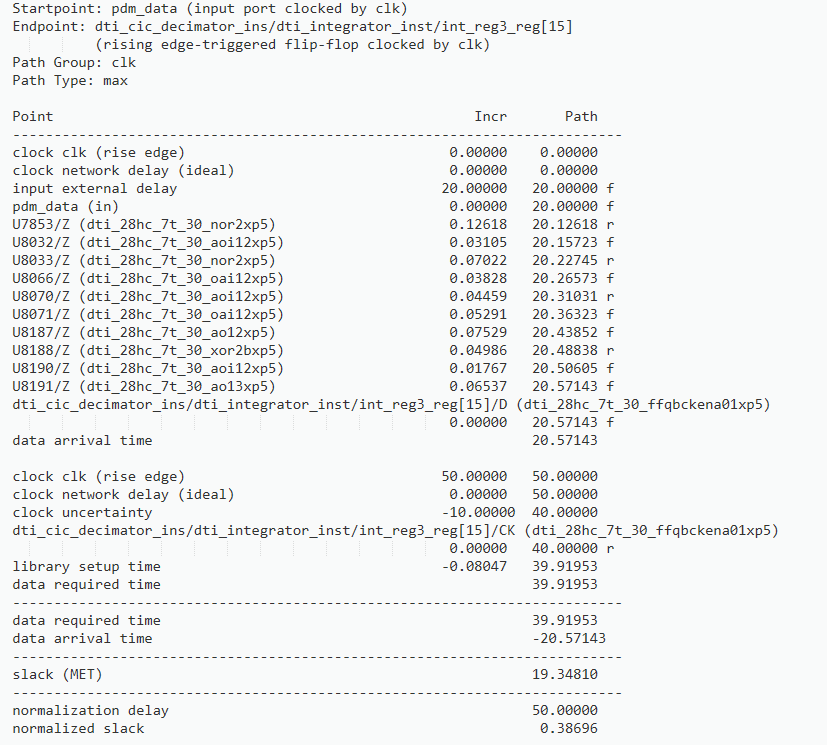
\includegraphics[width=12cm]{Images/Chuong5/syn/timing.png}
%     \caption[Báo cáo timing của thiết kế]{\bfseries \fontsize{12pt}{0pt}\selectfont Báo cáo timing của thiết kế}
%     \label{syn_t}
% \end{figure}

Với yêu cầu của bộ thiết là tần số chạy không cao (9216 kHz) thì về mặt timing không có gì cần phải quan tâm vì nó chắc chắn sẽ thỏa mãn. Thật vậy:
Đưa các ràng buộc về timing như sau:
\begin{itemize}
    \item Tần số tổng hợp: 20 MHz ($>$ 9216 kHz)
    \item Độ trễ đầu vào: cao nhất là 0.4 chu kỳ clock
    \item Độ trễ đầu đầu ra: cao nhất là 0.4 chu kỳ clock
\end{itemize}

Các thông số input delay và output delay được xác định khi ta ghép khối PDM2PCM 
với các khối khác trong hệ thống. Các khối khác chưa được hoàn thiện nên ta đặt các ràng buộc mang tính tương đối.

Báo cáo về mặt timing sẽ được mô tả ở bảng \ref{syn_t}. Ta thấy slack của critical path (đường có trễ cao nhất) đang dương rất lớn, từ đó có thể kết luận thiết kế thỏa mãn về timing.
\subsubsection{Tài nguyên sử dụng}

\begin{table}[H]
\centering
    \caption[Các báo cáo về mặt diện tích của thiết kế]{\bfseries \fontsize{12pt}{0pt}\selectfont Các báo cáo về mặt diện tích của thiết kế}
\begin{tabular}{|l|l|}
\hline
\multicolumn{1}{|c|}{\textbf{Thông tin}} &
  \multicolumn{1}{c|}{\textbf{\begin{tabular}[c]{@{}c@{}}Thông số\\ ($\mu m^2$)\end{tabular}}} \\ \hline
\begin{tabular}[c]{@{}l@{}}Diện tích phần tổ hợp\\ (Combinational area)\end{tabular}    & 1803.689998 \\ \hline
\begin{tabular}[c]{@{}l@{}}Diện tích phần buffer/inverter\\ (Buf/Inv area)\end{tabular} & 102.997997  \\ \hline
\begin{tabular}[c]{@{}l@{}}Diện tích phần không phải mạch tổ hợp\\ (Noncombinational area)\end{tabular} &
  3661.475934 \\ \hline
\begin{tabular}[c]{@{}l@{}}Diện tích phần hộp đen\\ (Macro/Black Box area)\end{tabular} & 0.000000    \\ \hline
Tổng cộng                                                                               & 5465.165932 \\ \hline
\end{tabular}
    \label{area}
    \end{table}

Bảng \ref{cell}, \ref{area} mô tả về mặt vật lý, nó chỉ rõ ra các số lượng port, net, các cell combinational và sequential. Từ đó đưa ra tổng diện tích của thiết kế.
Nhận thấy tổng diện tích 5465.165932 ($\mu m^2$) là trung bình ở mức chấp nhận được với những IP chuyển đổi.
\begin{table}[H]
\centering
    \caption[Các báo cáo về mặt số lượng phần tử của thiết kế]{\bfseries \fontsize{12pt}{0pt}\selectfont Các báo cáo về mặt số lượng phần tử của thiết kế}
    \begin{tabular}{|lc|l|}
\hline
\multicolumn{2}{|c|}{\textbf{Thông tin}}                    & \multicolumn{1}{c|}{\textbf{Số lượng}} \\ \hline
\multicolumn{2}{|l|}{Số port}                               & 29                                     \\ \hline
\multicolumn{2}{|l|}{Số lượng dây (nets)}                   & 6002                                   \\ \hline
\multicolumn{1}{|l|}{\multirow{2}{*}{Số cell}}   & Tuần tự  & 1664                                   \\ \cline{2-3} 
\multicolumn{1}{|l|}{}                           & Tổ hợp   & 4276                                   \\ \hline
\multicolumn{2}{|l|}{Số lượng hộp đen (macros/black boxes)} & 0                                      \\ \hline
\multicolumn{2}{|l|}{Số buffer/inveter}                     & 525                                    \\ \hline
\end{tabular}
    \label{cell}
    \end{table}

\subsubsection{Công suất}
% \begin{figure}[H]
%     \centering
%     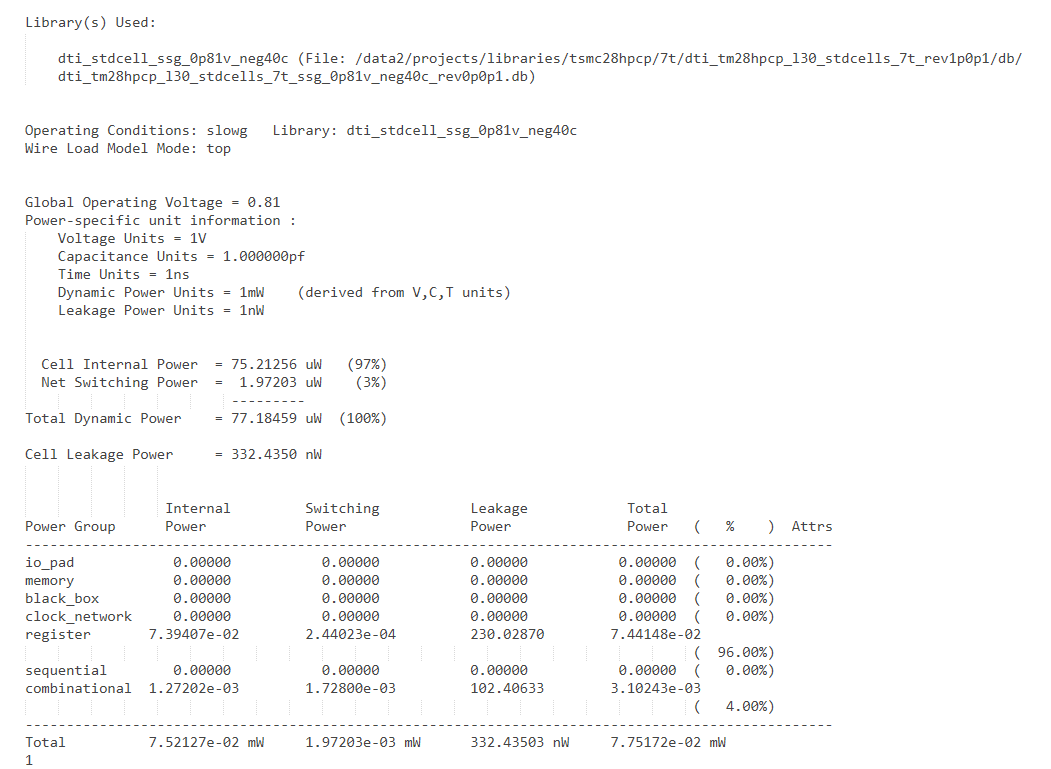
\includegraphics[width=14cm]{Images/Chuong5/syn/power.png}
%     \caption[Báo cáo công suất của thiết kế]{\bfseries \fontsize{12pt}{0pt}\selectfont Báo cáo công suất của thiết kế}
%     \label{syn_power}
% \end{figure}



Báo cáo về mặt công suất chỉ ra các thông số về mặt tiêu thụ năng nương, như năng 
lượng chuyển mạch, dòng dò, năng lượng bản thân cho các cell hoạt động. Báo cáo được mô tả như bảng \ref{syn_power}.
\begin{table}[H]
\centering
\caption[Báo cáo công suất của thiết kế]{\bfseries \fontsize{12pt}{0pt}\selectfont Báo cáo công suất của thiết kế}
\begin{tabular}{|l|l|}
\hline
\multicolumn{1}{|c|}{\textbf{Thông tin}} & \multicolumn{1}{c|}{\textbf{Giá trị}} \\ \hline
Internal Power & 7.52089e-02 (mW) \\ \hline
Switching Power & 1.97545e-03 (mW) \\ \hline
Leakage Power & 332.52689 (nW) \\ \hline
Tổng cộng & 7.75168e-02 (mW) \\ \hline
\end{tabular}
\label{syn_power}
\end{table}
\subsection{Triển khai thiết kế xuống FPGA}
Sau khi hoàn thành mô phỏng và tổng hợp, đảm bảo thiết kế hoạt động đúng chức 
năng yêu cầu. Để đảm bảo thiết kế hoạt động ổn định trong các thiết bị thực tế thì chúng ta sẽ triển khai thiết kế xuống FPGA.

\textbf{Giới thiệu về kit phát triển Zedboard} (hình \ref{zedboard}):

Zedboard được thiết kế trên nền tảng của một vi xử lý ARM Cortex-A9 MPCore lõi kép của Xilinx, với các tính năng khác như bộ nhớ DDR3, kết nối Ethernet, USB và các cổng giao tiếp khác như PMOD và FMC. Zedboard cũng được trang bị một FPGA Xilinx 7 series để cho phép người dùng tùy chỉnh phần cứng và thiết kế các hệ thống phức tạp.

\begin{figure}[H]
    \centering
    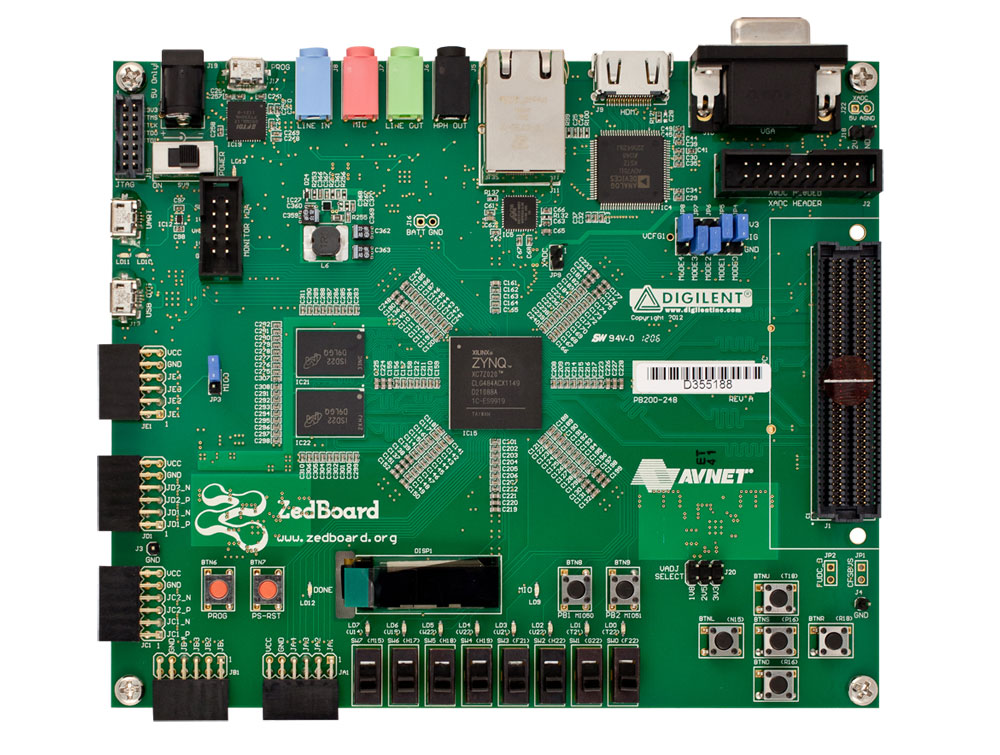
\includegraphics[width=12cm]{Images/Chuong5/fpga/zedboard.jpg}
    \caption[Kit ZedBoard]{\bfseries \fontsize{12pt}{0pt}\selectfont Kit ZedBoard}
    \label{zedboard}
\end{figure}

Zedboard được thiết kế trên nền tảng của một vi xử lý ARM Cortex-A9 MPCore lõi kép của Xilinx, với các tính năng khác như bộ nhớ DDR3, kết nối Ethernet, USB và các cổng giao tiếp khác như PMOD và FMC. 


Kit phát triển Zedboard được thiết kế để hỗ trợ các phần mềm như Xilinx SDK và Vivado Design Suite, cho phép người dùng thiết kế phần cứng và phần mềm cùng một lúc trên một nền tảng. Điều này giúp tăng hiệu suất và tối ưu hóa thiết kế phần cứng và phần mềm.

Với các tính năng và khả năng linh hoạt của nó, Zedboard là một công cụ hữu ích cho các kỹ sư và nhà phát triển trong việc phát triển các hệ thống nhúng phức tạp và đòi hỏi sự tùy chỉnh cao.



\subsubsection{Thiết kế bộ bao để triển khai trên hệ thống SOC} \label{wrapper_cha}

Để triển khai thiết kế lên hệ thống SOC (System On Chip), chúng ta cần sử dụng một bộ điều khiển để xử lý và đọc dữ liệu của đầu ra PCM, sau đó lưu vào một vùng nhớ có địa chỉ cố định. Từ địa chỉ đó vi xử lý mới có thể đọc dữ liệu về và làm những bước tiếp theo. Hình \ref{wrapper} mô tả kiến trúc của bộ bao (pdm2pcm\_warpper) nó sử dụng chuẩn giao tiếp APB (Advanced Peripheral Bus) -  1 chuẩn giao tiếp rất phổ biến trong hệ thống SOC dùng để giao tiếp với ngoại vi.

\begin{figure}[H]
    \centering
    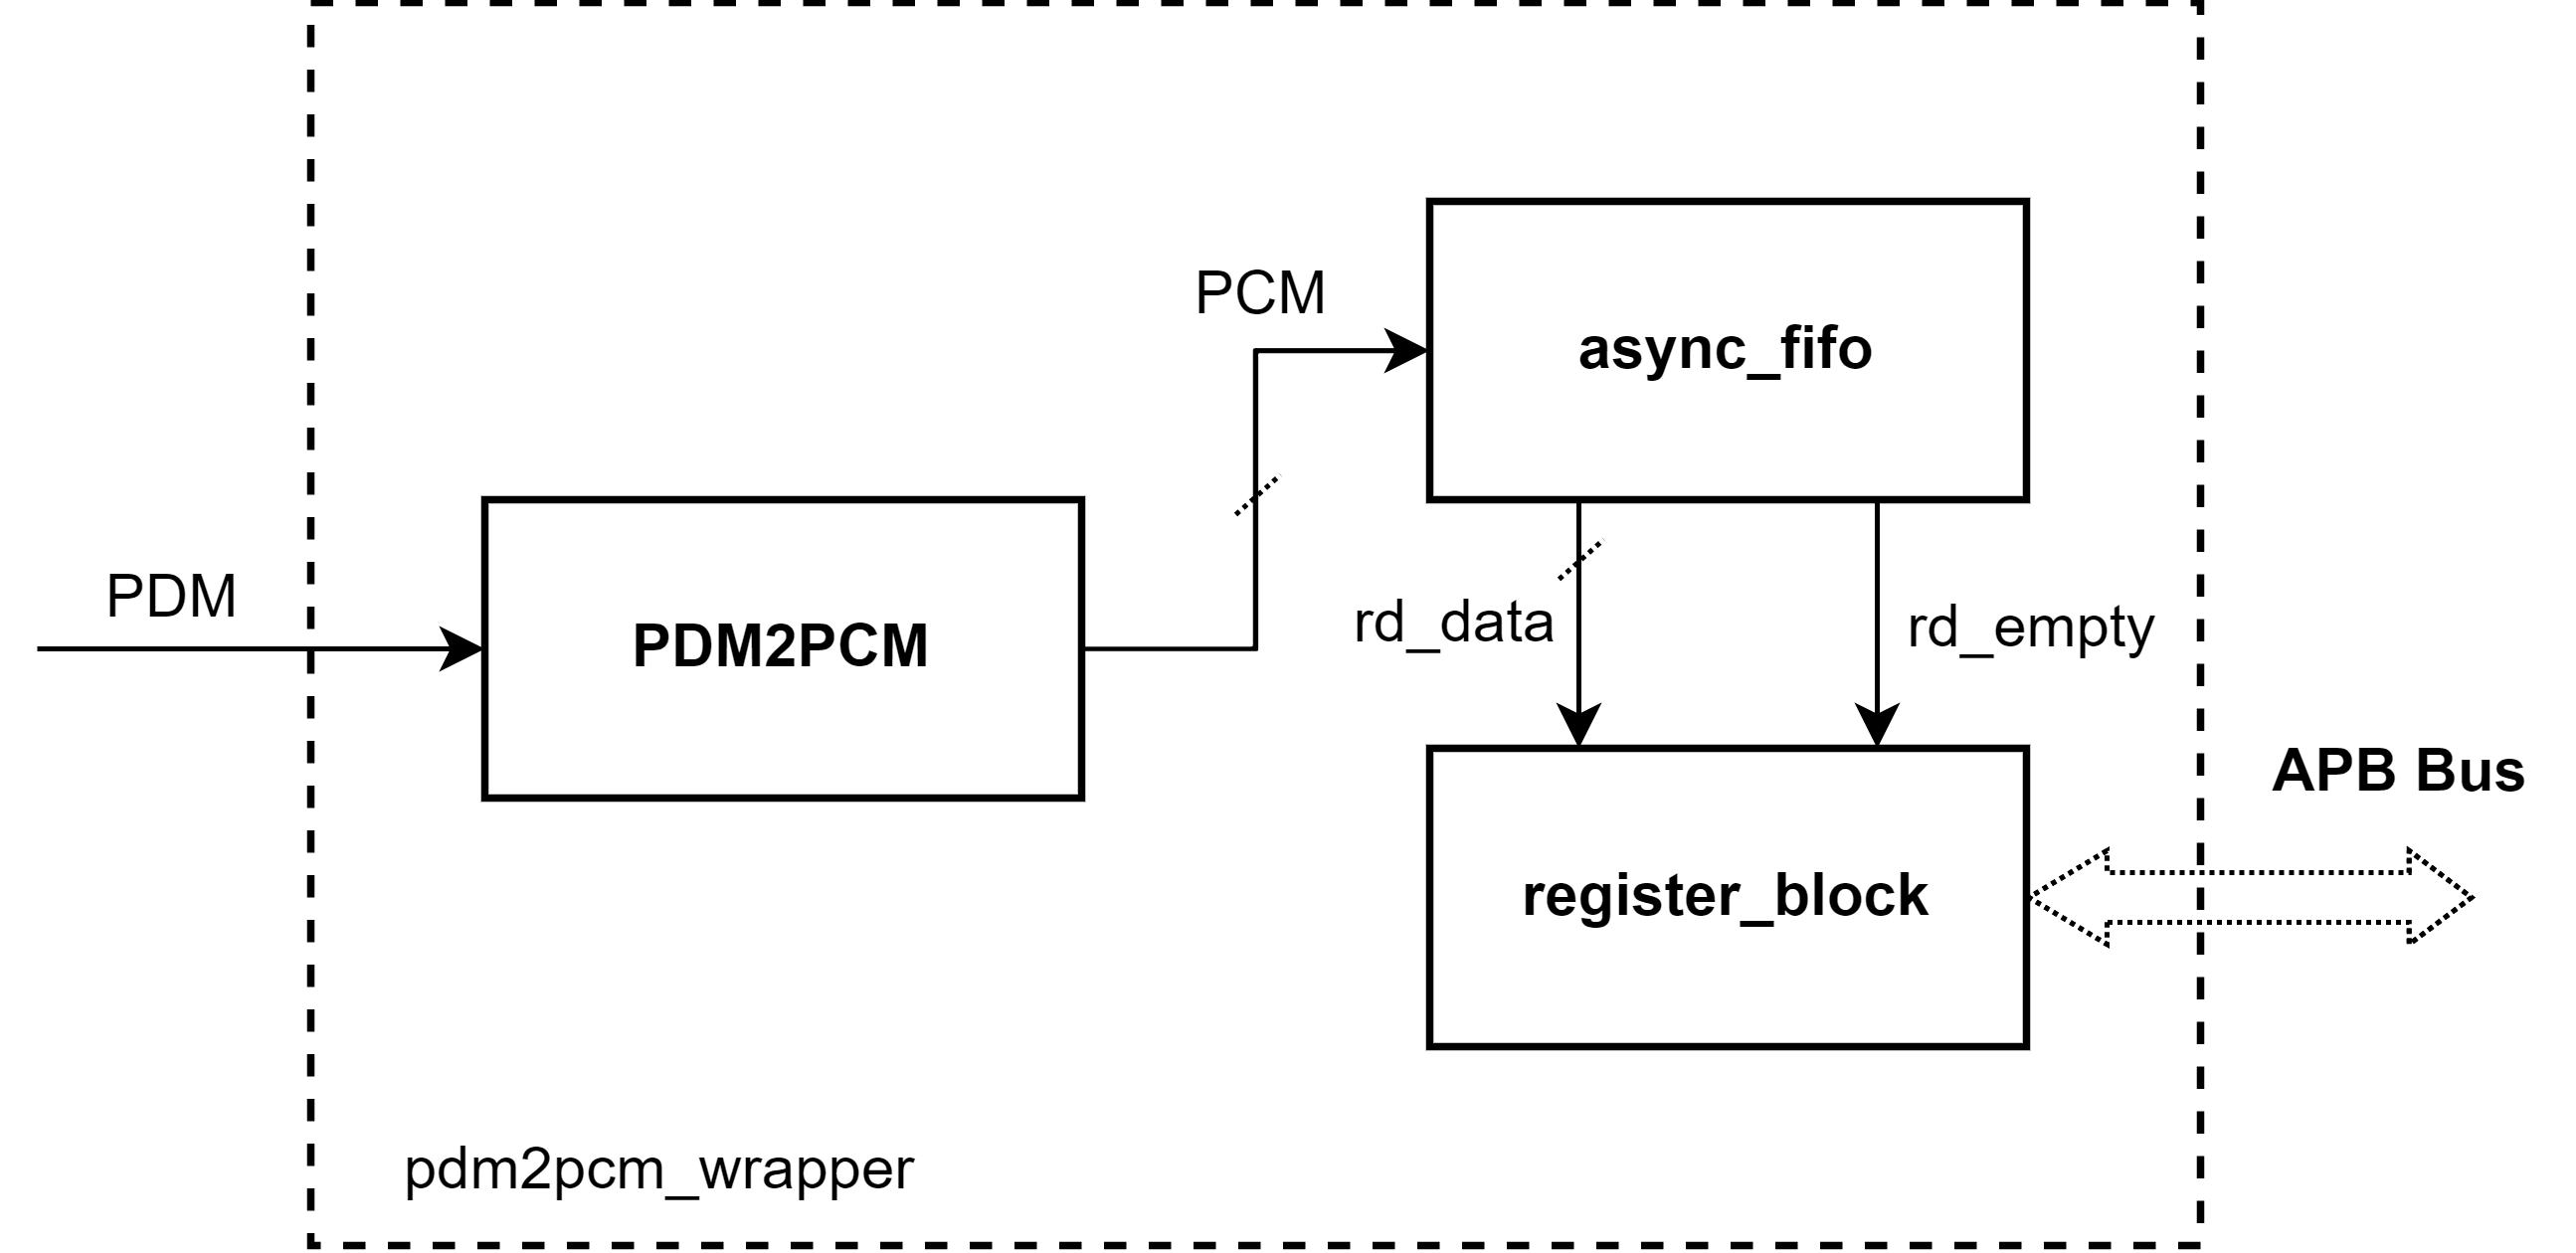
\includegraphics[width=13cm]{Images/Chuong5/fpga/wrapper.png}
    \caption[Sơ đồ khối của bộ pdm2pcm\_warpper]{\bfseries \fontsize{12pt}{0pt}\selectfont Sơ đồ khối của bộ pdm2pcm\_warpper}
    \label{wrapper}
\end{figure}

Khối \textbf{register\_block} đóng vai trò trung chuyển dữ liệu từ pdm2pcm lên vi xử lý. Nó lưu 2 giá trị PCM đầu ra và trạng thái trống của bộ đệm. Nó có cấu trúc như hình \ref{bit}. Thiết kế này chỉ lấy 16bit PCM và sẽ được phát trên 2 kênh trái và phải của loa.

\begin{figure}[H]
    \centering
    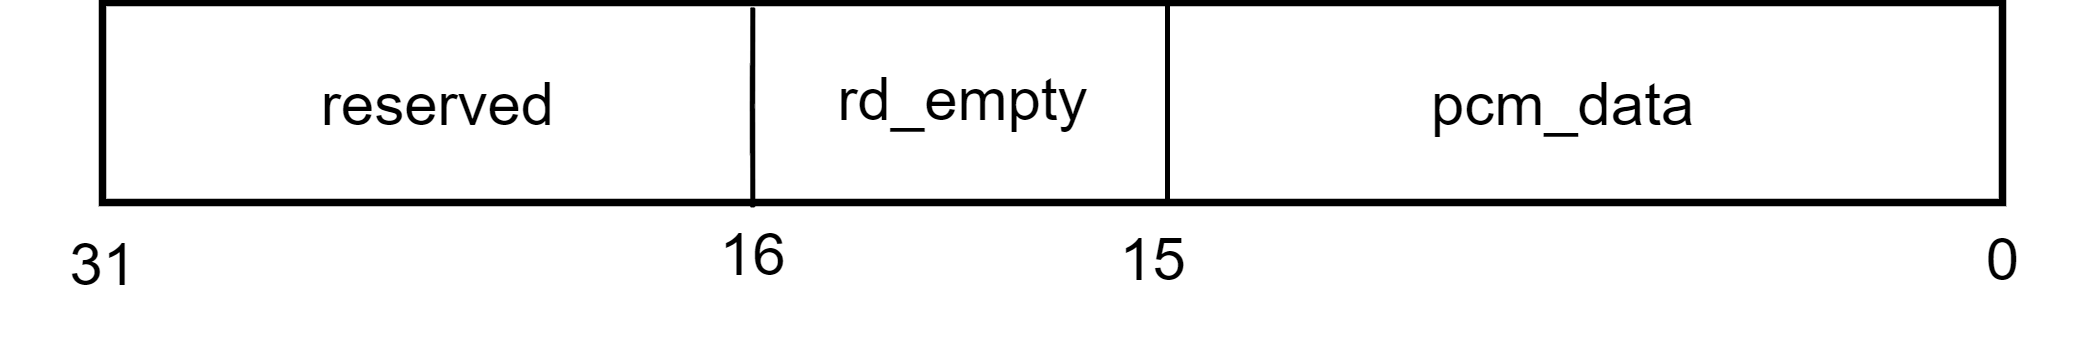
\includegraphics[width=9cm]{Images/Chuong5/fpga/bit.png}
    \caption[Sơ đồ khối của bộ pdm2pcm\_warpper]{\bfseries \fontsize{12pt}{0pt}\selectfont Sơ đồ khối của bộ pdm2pcm\_warpper}
    \label{bit}
\end{figure}

Lúc này vi xử lý có thể biết lúc nào có thể đọc (có dữ liệu) thông qua thanh ghi rd\_empty, khi đó dữ liệu đã có sẵn trên thanh ghi pcm\_data và có thế đọc. Các giá trị trong thanh ghi sẽ được cập nhật liên tục với tần số của hệ thống chính.

Vì thiết kế sử dụng tần số khác với tần số của hệ thống (2 miền tần số) sẽ dẫn đến thất lạc dữ liệu ở 1 số thời điểm, điều đó gây mất chính xác của hệ thống. Để  sai sót này, chúng ta sẽ chèn 1 bộ đệm không đồng bộ để đồng bộ hai miền tần số. Tất cả các dữ liệu đầu ra PCM sẽ được ghi liên tục vào \textbf{async\_fifo} và tất nhiên lúc fifo đầy sẽ dừng. Bộ fifo sẽ nhận được tín hiệu đọc dữ liệu ra thông qua các sự kiện đọc từ vi xử lý thông qua bus APB, lúc này trên \textbf{register\_block} sẽ cập nhật giá trị mới. Tín hiệu rd\_empty cũng báo cho hệ thống là bộ lọc đang hay không có dữ liệu, điều này là hết sức cần thiết để thông báo cho vi xử lý biến lúc nào cần lấy dữ liệu.

\subsubsection{Ý tưởng thiết kế}

Tín hiệu PDM sẽ được tạo ra từ micro MEMS được bán trên thị trường. Ý tưởng ở đây là hệ thống đọc tín hiệu từ micro và sau đó phát qua loa một trong thời gian thực.
Ý tưởng mô tả như hình hình \ref{pinouts}.
\begin{figure}[H]
    \centering
    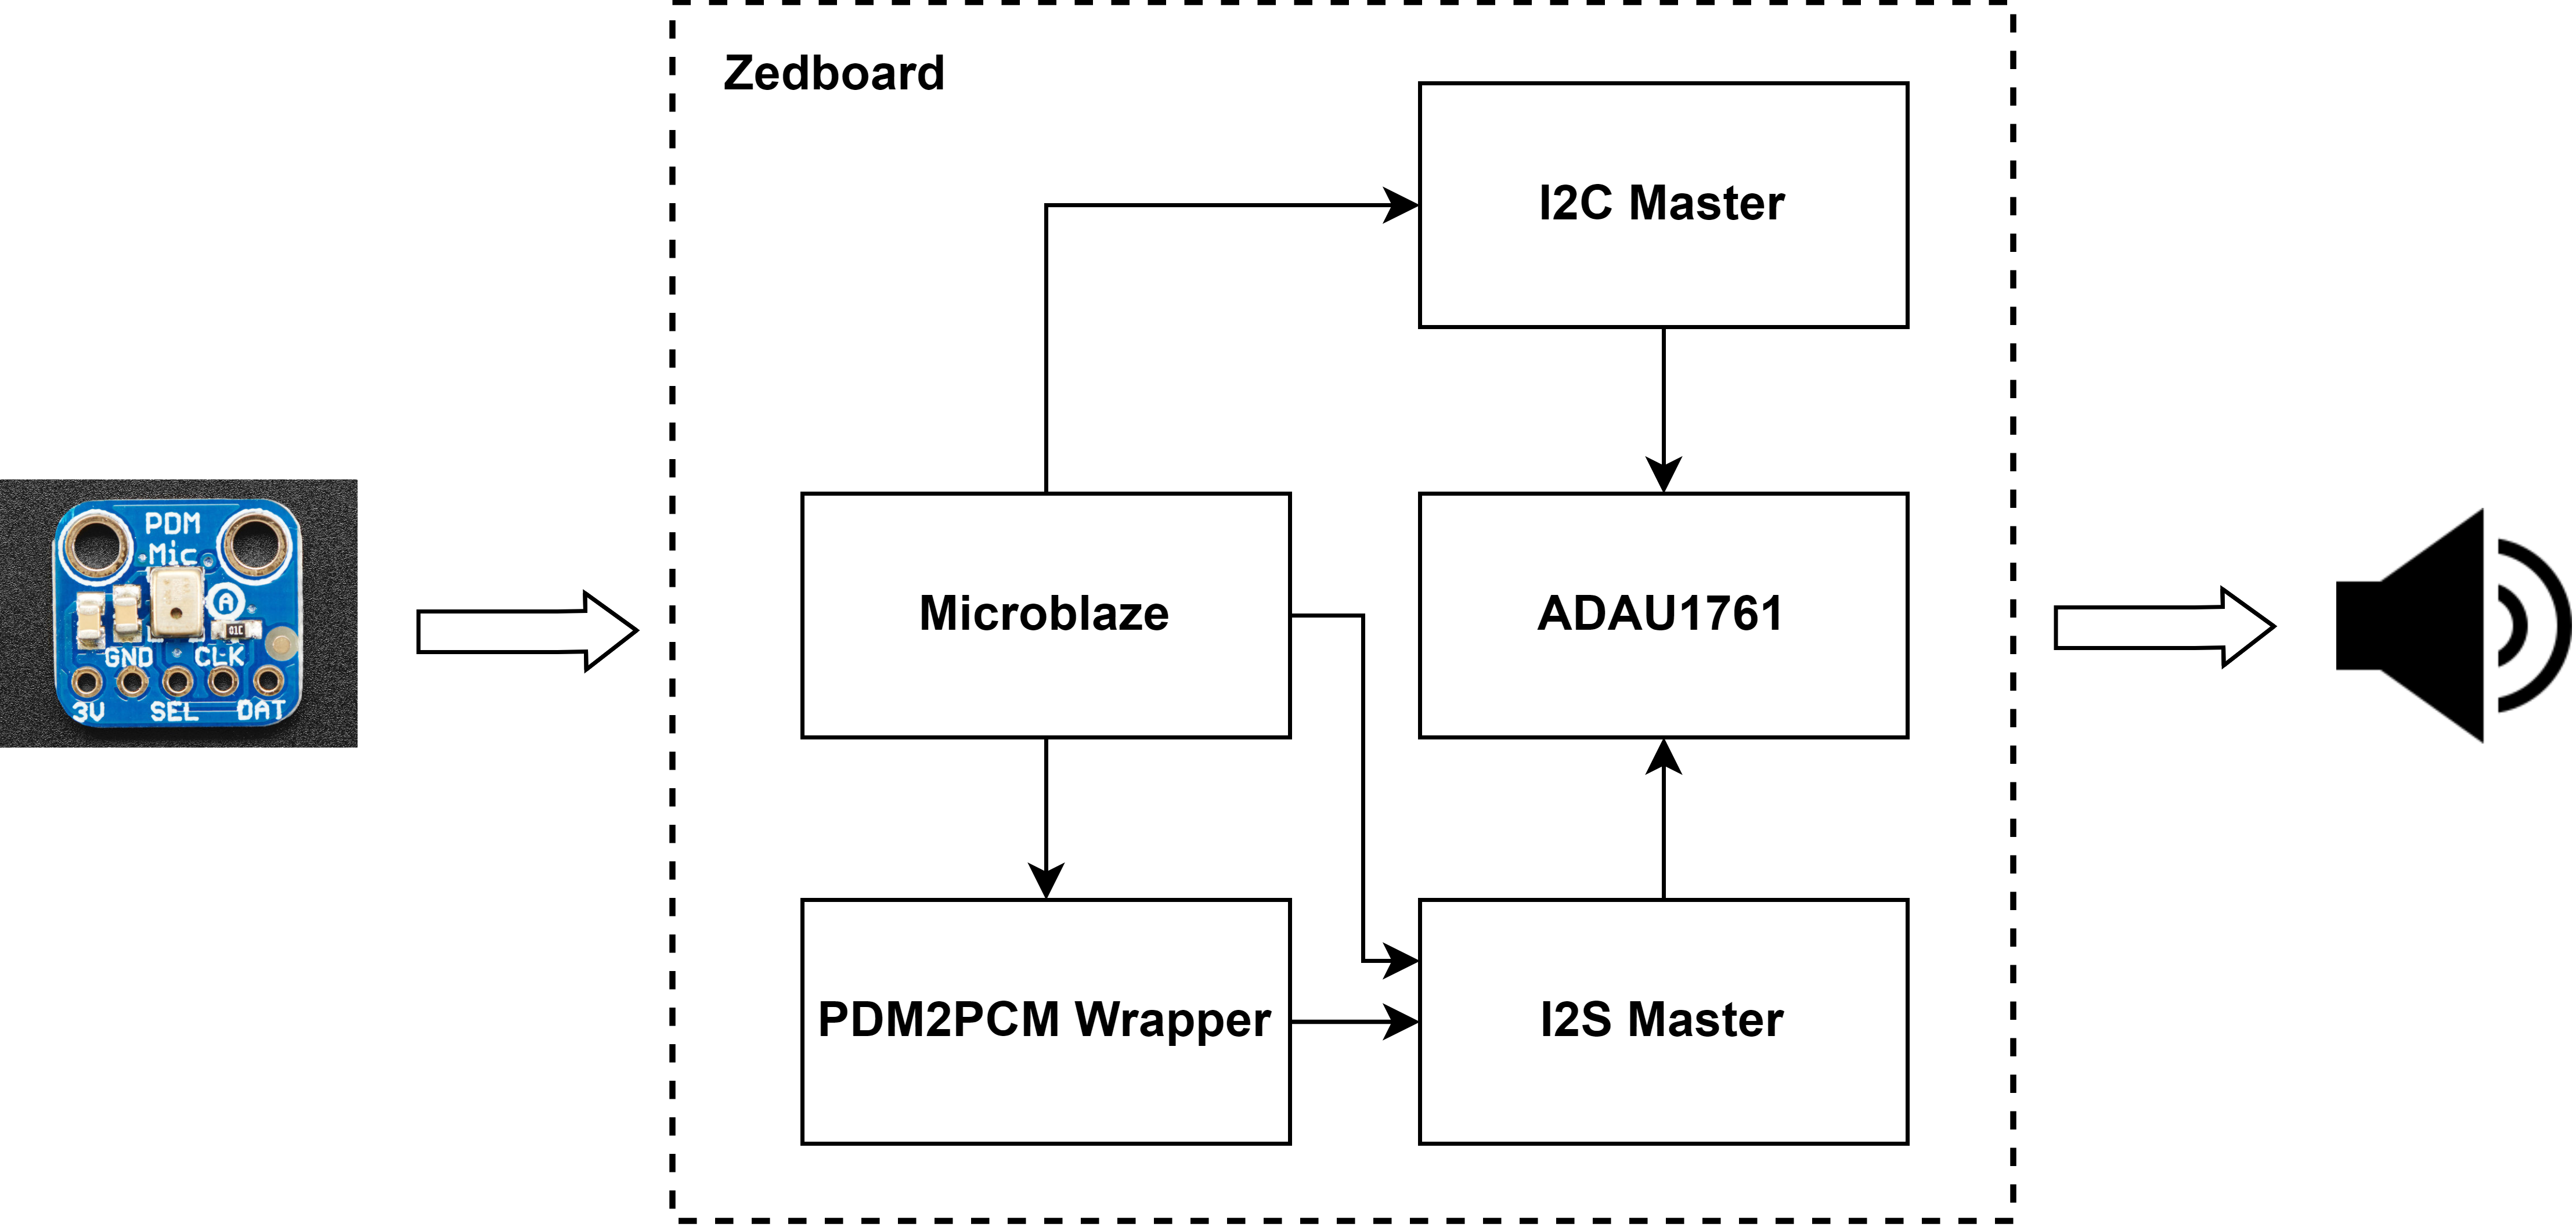
\includegraphics[width=14cm]{Images/Chuong5/fpga/top.png}
    \caption[Sơ đồ ý tưởng của thiết kế]{\bfseries \fontsize{12pt}{0pt}\selectfont Sơ đồ ý tưởng của thiết kế}
    \label{pinouts}
\end{figure}

Trên kit Zedboard đã có sẵn bộ I2S Audio CODEC - ADAU1761, nó sẽ được tận dụng để phát âm thanh ra loa. Chúng ta sẽ sử dụng thêm bộ I2S master để chuyển đổi tín hiệu PCM thành I2S sau đó dùng ADAU1761 để chuyển đổi sang tín hiệu tương tự và phát ra loa. Điều đáng chú ý ở đây, ADAU1761 được cấu hình các thông số thông qua giao tiếp SPI hoặc I2C vì vậy chúng ta sẽ sử dụng thêm bộ I2C master để làm việc này. Sơ đồ khối chi tiết và cách làm việc sẽ được trình bày ở mục tiếp theo.

Để kiểm soát toàn bộ các quá trình gửi và nhận dữ liệu từ PC, bộ xử lí MicroBlaze được sử dụng để làm trung gian điều phối quá trình gửi và nhận dữ liệu

Hình \ref{adau} mô tả kiến trúc bên trong của IC ADAU1761. Đầu ra âm thanh của nó có 2 kênh (stereo) được xử lý hoàn toàn riêng biệt với nhau. Bộ \textbf{PLL} để tạo ra các tần số cần dùng. Khối \textbf{Serial Data} thực chất là I2S slave, nó thu nhận tín hiệu sau đó gửi đến các bộ lọc để đưa tín hiệu ra các kênh. Việc cấu hình thiết bị sẽ do bộ \textbf{I2S/SPI Control Port} xử lý.

\begin{figure}[H]
    \centering
    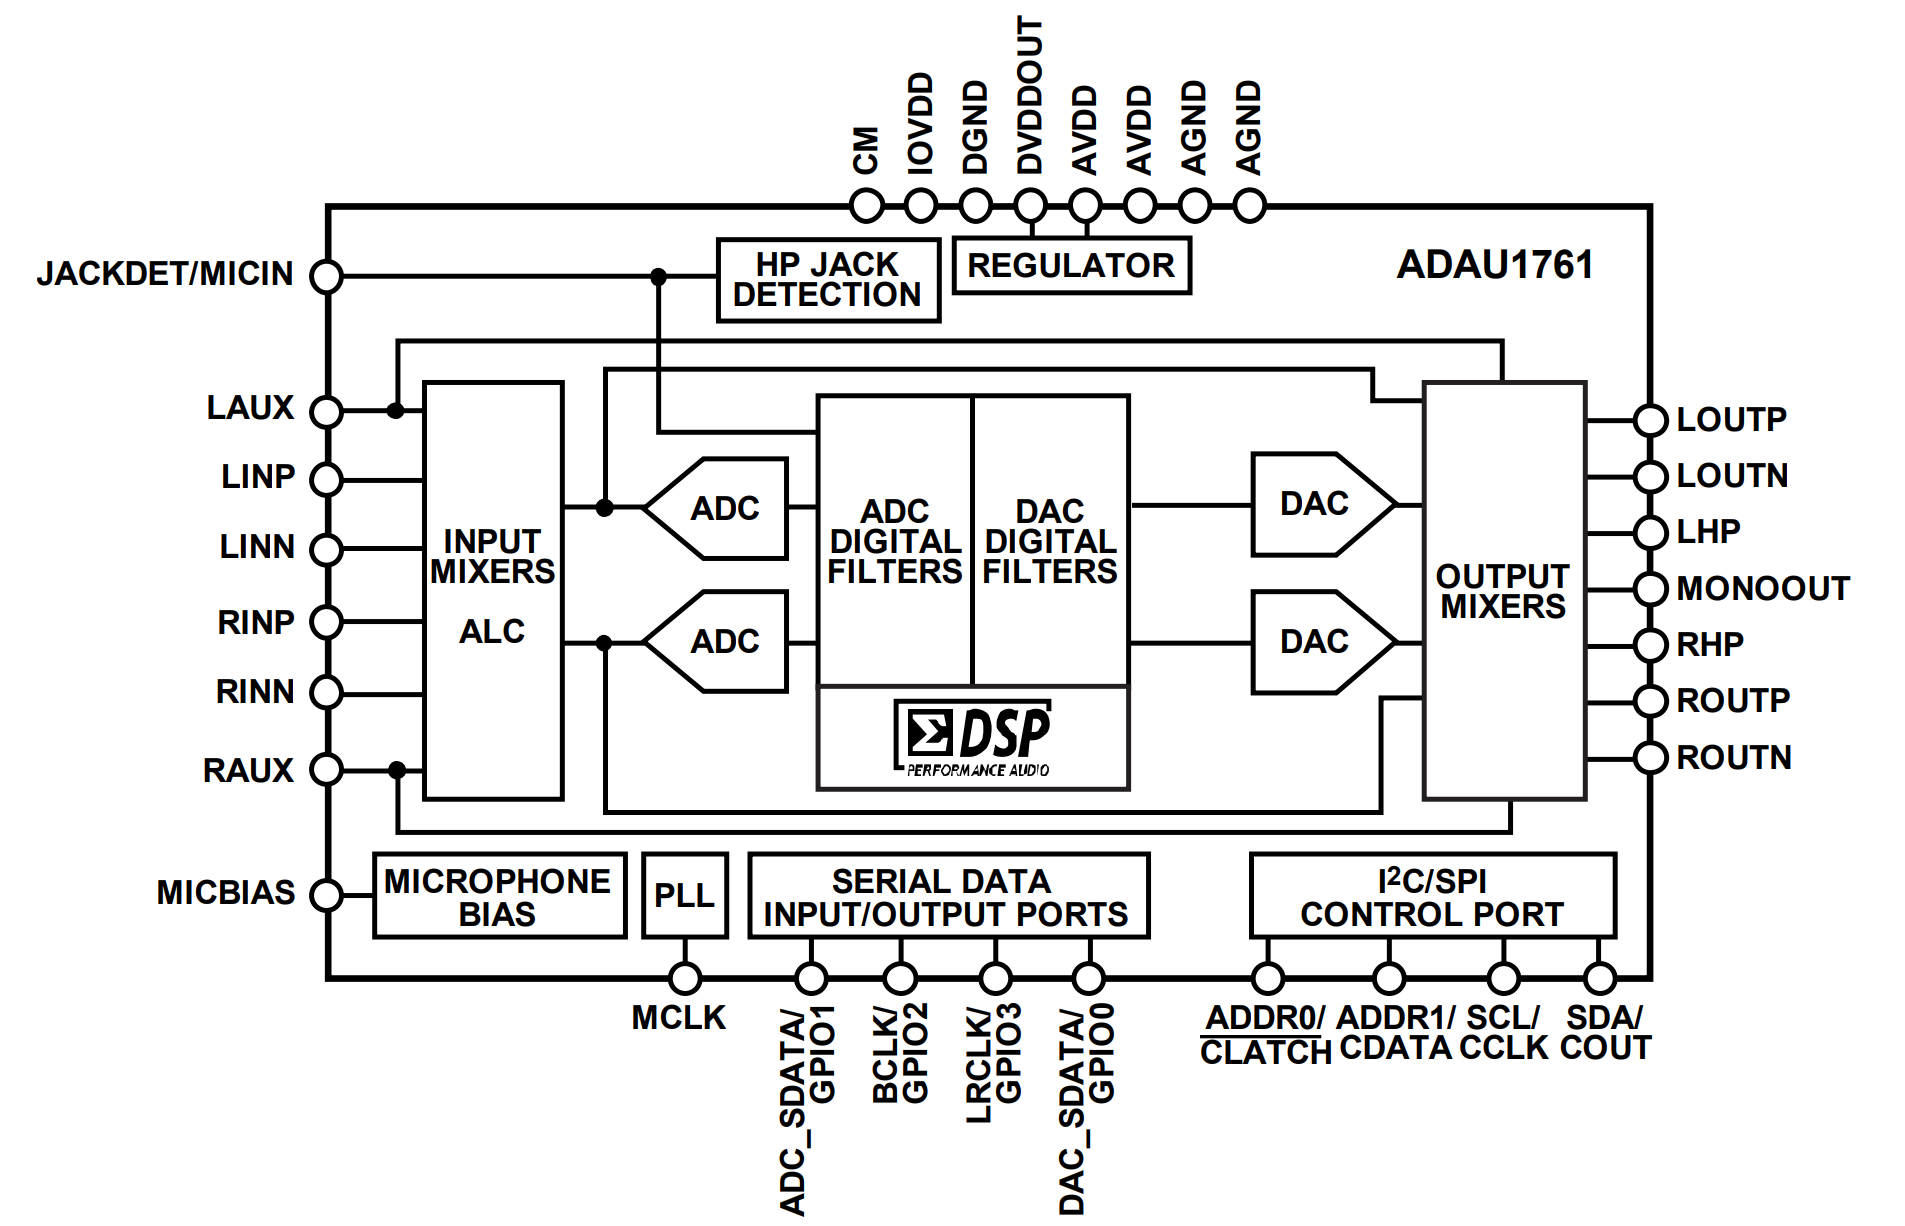
\includegraphics[width=14cm]{Images/Chuong5/fpga/adau.png}
    \caption[Sơ đồ khối của ADAU1761]{\bfseries \fontsize{12pt}{0pt}\selectfont Sơ đồ khối của ADAU176}
    \label{adau}
\end{figure}



\subsubsection{Triển khai trên trên phần mềm Vivado}

Kit phát triển Zedboard được thiết kế để hỗ trợ các phần mềm như Xilinx SDK và Vivado Design Suite, cho phép người dùng thiết kế phần cứng và phần mềm cùng một lúc trên một nền tảng,  giúp tăng hiệu suất và tối ưu hóa thiết kế phần cứng và phần mềm.

Do sử dụng kit trong đề tài này là Zedboard đồng nghĩa với việc chúng ta phải thực hiện tất cả các quá trình trên phần mềm Vivado - một nền tảng phát triển của \textbf{Xilinx}.
Quy trình thực hiện sẽ bao gồm các bước như sau:
\begin{enumerate}
    \item Tạo dự án: chọn kit sử dụng, ...
    \item Pakage tất cả các IP: I2S, I2C, pdm2pcm\_wrapper
    \item Viết driver code bằng ngôn ngữ C
    \item Mô phỏng thiết kế qua phần mềm QuestaSim
    \item Gán chân vào ra ứng với các cổng trên kit
    \item Tổng hợp
    \item Triển khai thiết kế
    \item Tạo bitstream
    \item Nạp xuống kit
\end{enumerate}



\paragraph{Thiết kế block design}

\begin{figure}[H]
    \centering
    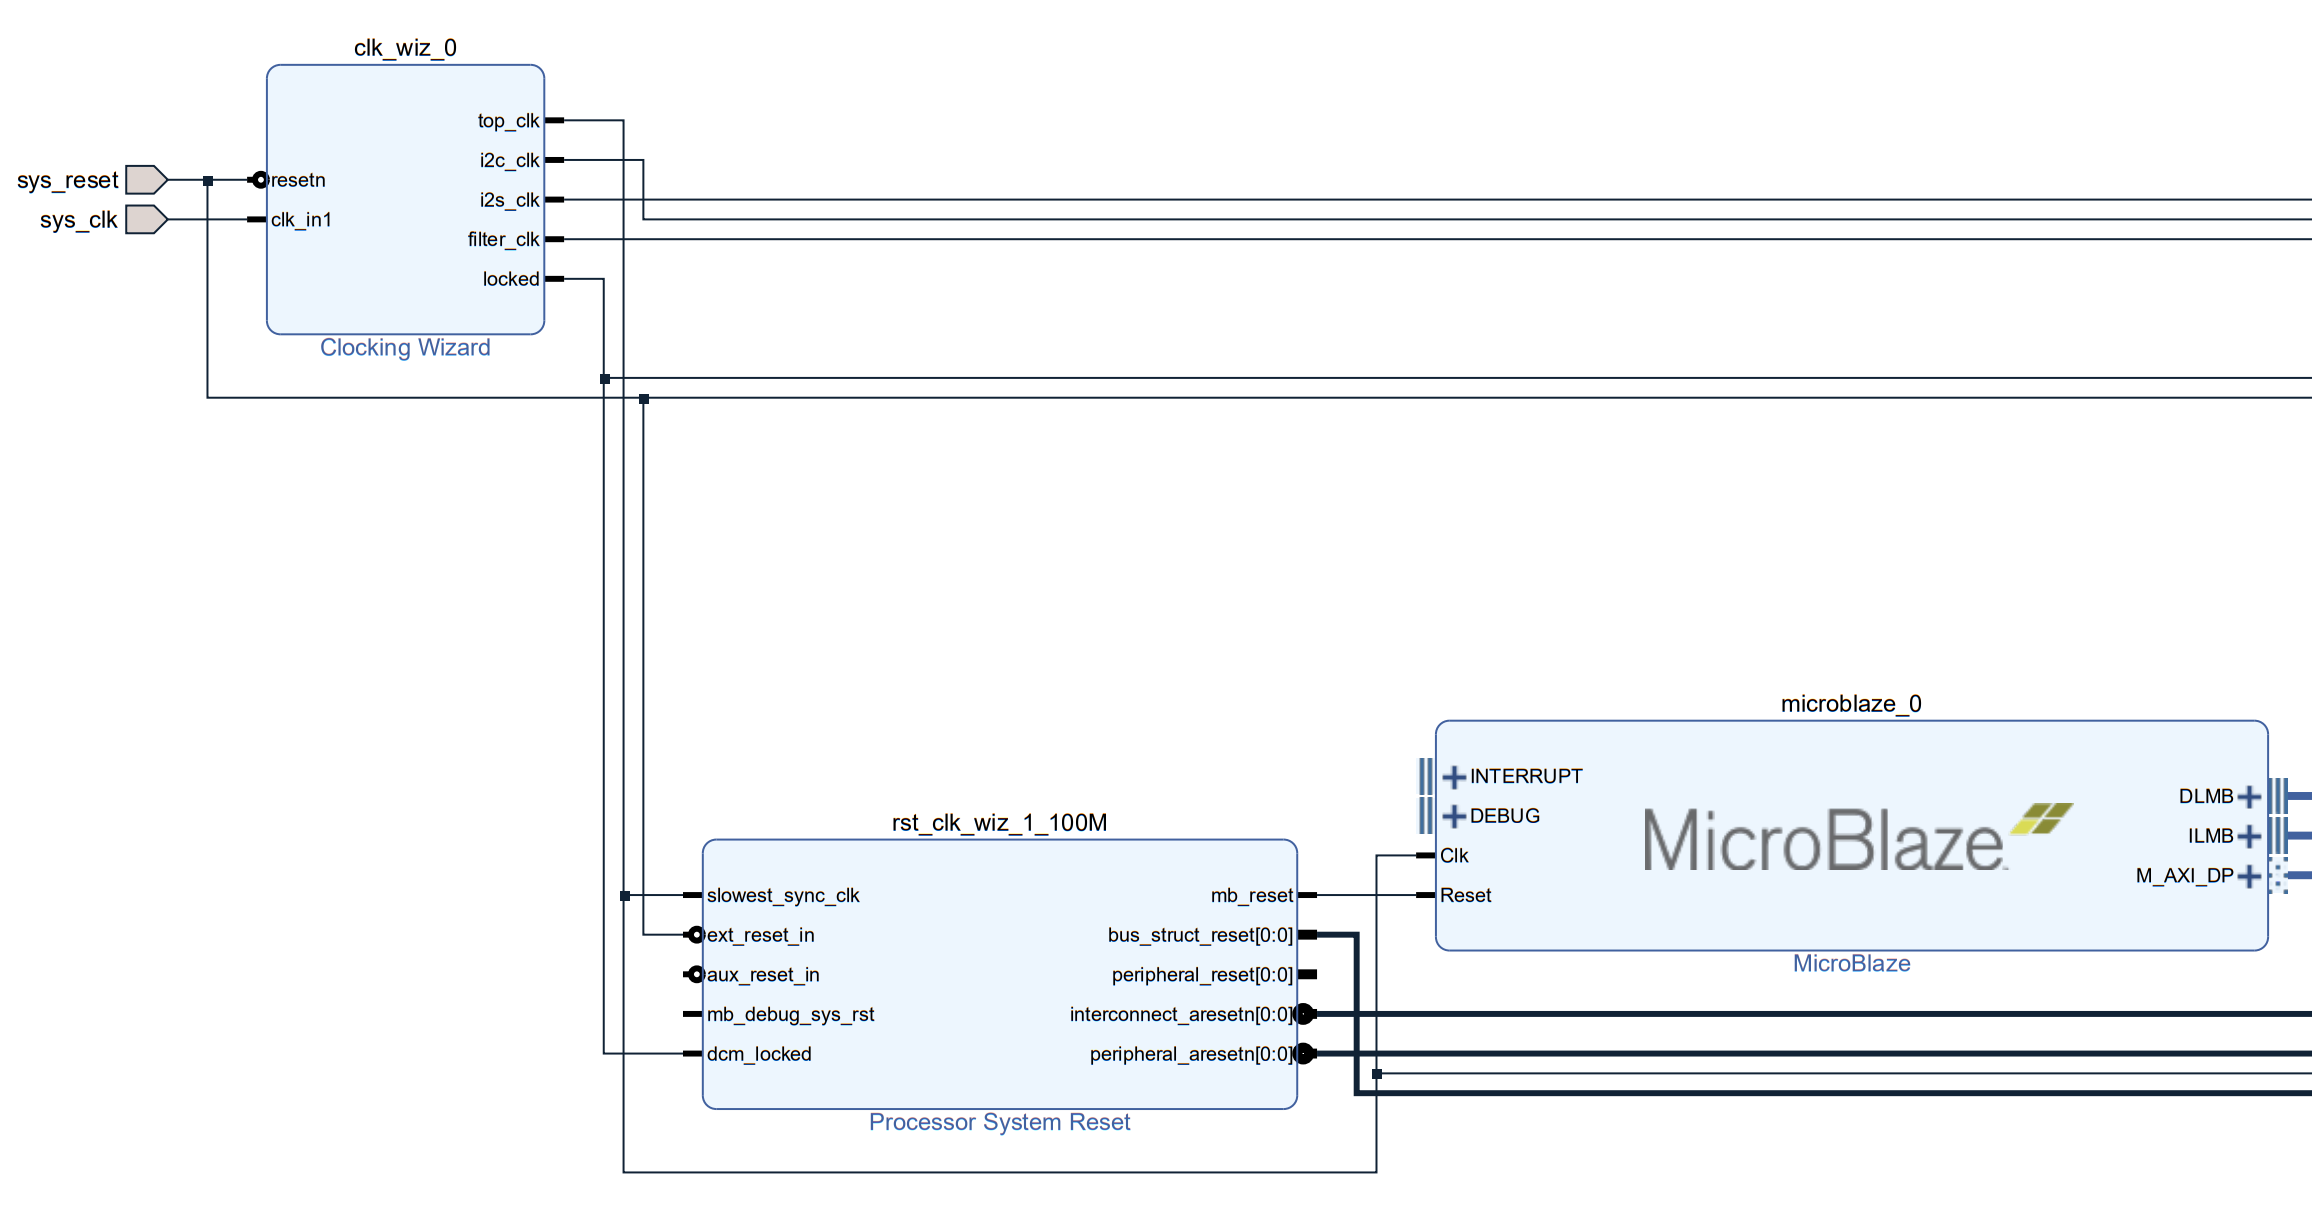
\includegraphics[width=15cm]{Images/Chuong5/fpga/block_design_1.png}
    \caption[Block design của hệ thống]{\bfseries \fontsize{12pt}{0pt}\selectfont Block design của hệ thống}
    \label{bd1}
\end{figure}

\begin{figure}[H]
    \centering
    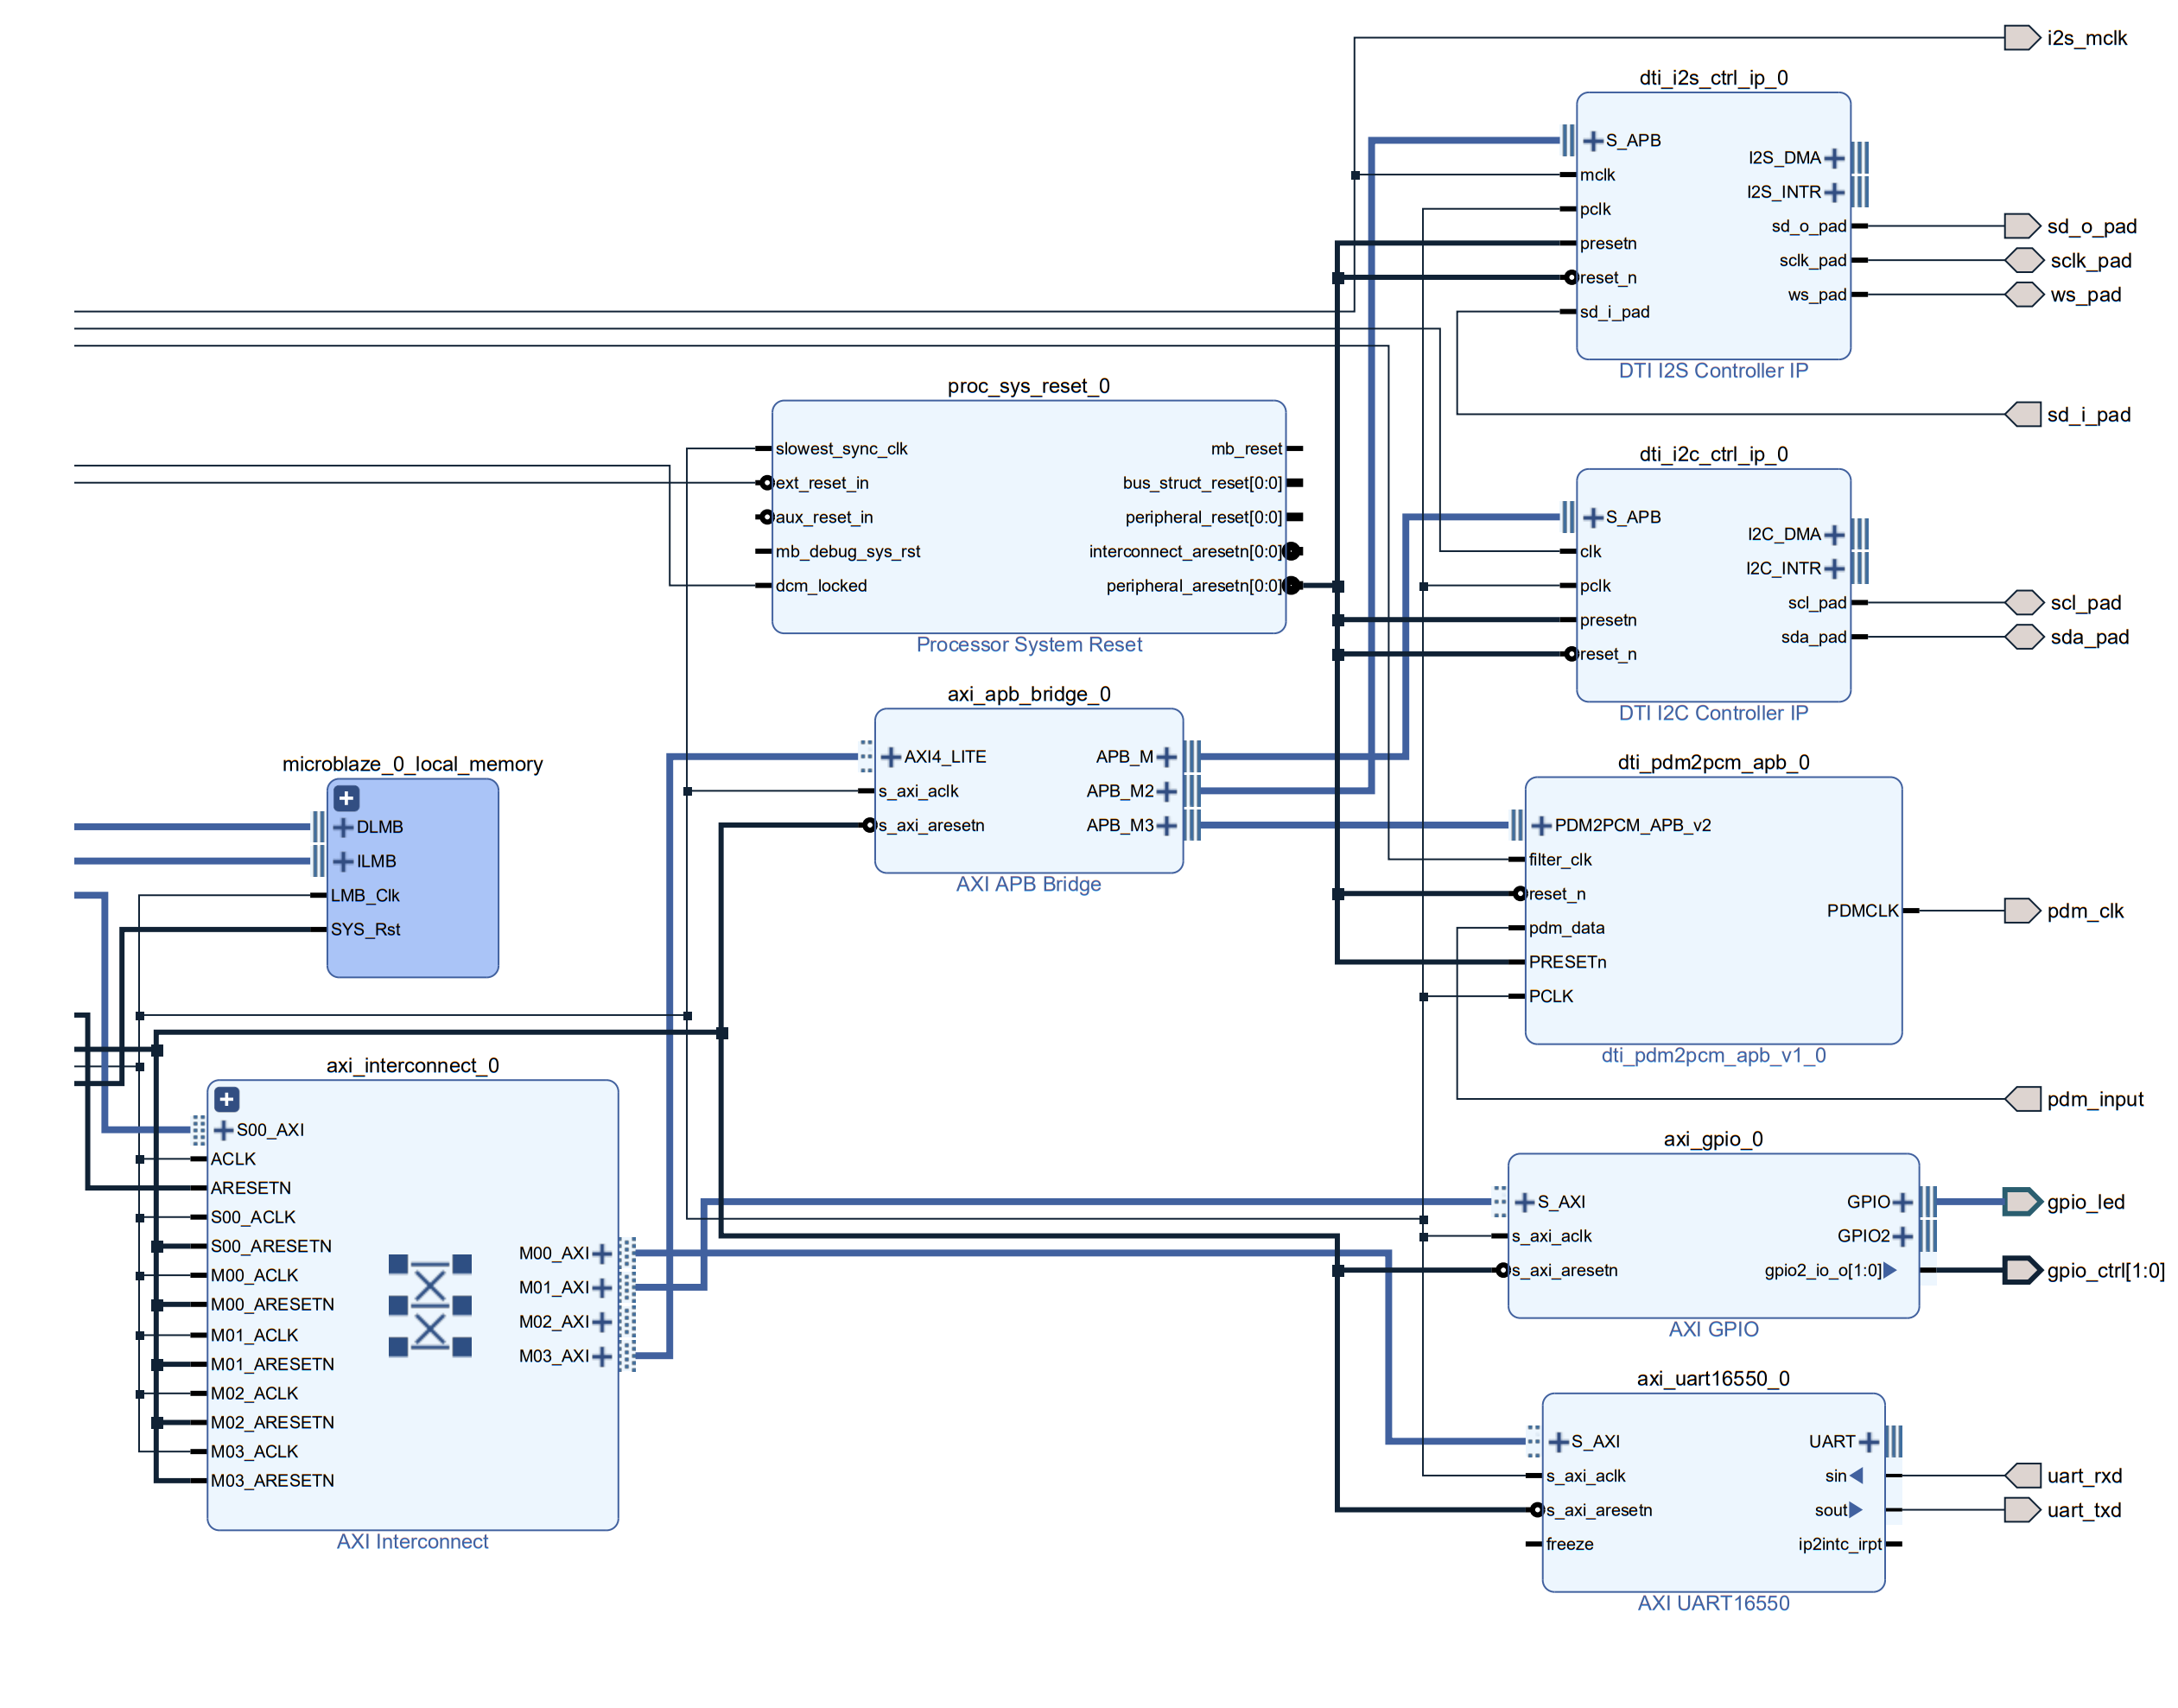
\includegraphics[width=15cm]{Images/Chuong5/fpga/block_design_2.png}
    \caption[Block design của hệ thống (tiếp)]{\bfseries \fontsize{12pt}{0pt}\selectfont Block design của hệ thống (tiếp)}
    \label{bd2}
\end{figure}
Hình \ref{bd1}, \ref{bd2} mô tả block design của hệ thống. Với bộ não trung tâm là vi xử lý MicroBlaze (\textbf{microblaze\_0}) đảm nhận vai trò đọc ghi và xử lý dữ liệu. Bộ Clock Wizard (\textbf{clk\_wir\_0}) thực hiện tạo ra các tần số mong muốn, ở đây ta có top\_clk ứng với tần số 50 MHz cung cấp cho toàn bộ hệ thống, i2s\_clk là tần số cấp cho bộ I2S với giá trị 36.864 MHz và tần số cấp cho bộ lọc filter\_clk là 9.216 Mhz.

 Khối \textbf{axi\_interconnect\_0} đảm nhận việc ánh xạ một thiết bị master AXI ra nhiều slave AXI. Hệ thống sử dụng chuẩn AXI để làm interconnect (AXI Interconnect), bộ này quản lý (phân địa chỉ) tất cả các ngoại vi. Nó được xem là bộ điều khiển sao cho việc truy xuất dữ liệu đúng với yêu cầu từ vi xử lý.

Khối \textbf{axi\_apb\_bridge}, \textbf{microblaze\_0} giao tiếp theo chuẩn AXI còn các lõi 
thiết kế thì giao tiếp bằng chuẩn APB nên cần một khối có thể chuyển đổi các chuẩn 
giao tiếp này
% \newpage


Bộ \textbf{AXI UART 16550} dùng để truyền và nhận dữ liệu thông qua chuẩn UART. Nó là cổng trung gian để kết nối với PC, từ đây PC có thể đọc được dữ liệu từ hệ thống, thông thường sẽ đi kèm với câu lênh \textit{printf(char*)}.

Bộ \textbf{dti\_pdm2pcm\_apb\_0} là bộ bao đã được thiết kế ở mục \ref{wrapper_cha}. Nó sử dụng chuẩn APB thực hiện đọc ghi dữ liệu, nên để kết nối với vi xử lý chúng ta cần thêm 1 bộ cầu nối để dùng chuẩn AXI.

\textbf{DTI I2S Controller IP} và \textbf{DTI I2C Controller IP} lần lượt là I2S master và I2C master, tất cả các IP đều được do công ty \textbf{Dolphin Tecnology VietNam Center} phát triển. Chúng sử dụng giao thức APB để cấu hình cũng như điều khiển truyền dữ liệu.
\begin{table}[H]
\centering
    \caption[Sắp xếp địa chỉ trong block design]{\bfseries \fontsize{12pt}{0pt}\selectfont Sắp xếp địa chỉ trong block design}
    \begin{tabular}{|lllllll}
\hline
\multicolumn{2}{|c|}{\textbf{Tên}} &
  \multicolumn{1}{c|}{\textbf{\begin{tabular}[c]{@{}c@{}}Giao diện \\ Slave\end{tabular}}} &
  \multicolumn{1}{c|}{\textbf{Kiểu}} &
  \multicolumn{1}{c|}{\textbf{Địa chỉ offset}} &
  \multicolumn{1}{c|}{\textbf{\begin{tabular}[c]{@{}c@{}}Phạm \\ vi\end{tabular}}} &
  \multicolumn{1}{c|}{\textbf{Địa chỉ cao nhất}} \\ \hline
\multicolumn{7}{|l}{Dữ liệu - Data (32 address bits : 4G)} \\ \hline
 &
  \multicolumn{1}{l|}{GPIO} &
  \multicolumn{1}{l|}{S\_AXI} &
  \multicolumn{1}{l|}{Reg} &
  \multicolumn{1}{l|}{0x4000\_0000} &
  \multicolumn{1}{l|}{64K} &
  \multicolumn{1}{l|}{0x4000\_FFFF} \\ \hline
 &
  \multicolumn{1}{l|}{UART 16550} &
  \multicolumn{1}{l|}{S\_AXI} &
  \multicolumn{1}{l|}{Reg} &
  \multicolumn{1}{l|}{0x44A0\_0000} &
  \multicolumn{1}{l|}{64K} &
  \multicolumn{1}{l|}{0x44A0\_FFFF} \\ \hline
 &
  \multicolumn{1}{l|}{Local Memory} &
  \multicolumn{1}{l|}{SLMB} &
  \multicolumn{1}{l|}{Mem} &
  \multicolumn{1}{l|}{0x0000\_0000} &
  \multicolumn{1}{l|}{32K} &
  \multicolumn{1}{l|}{0x0000\_7FFF} \\ \hline
 &
  \multicolumn{1}{l|}{I2C Controller} &
  \multicolumn{1}{l|}{S\_APB} &
  \multicolumn{1}{l|}{Reg} &
  \multicolumn{1}{l|}{0x44A2\_0000} &
  \multicolumn{1}{l|}{64K} &
  \multicolumn{1}{l|}{0x44A2\_FFFF} \\ \hline
 &
  \multicolumn{1}{l|}{I2S Controller} &
  \multicolumn{1}{l|}{S\_APB} &
  \multicolumn{1}{l|}{Reg} &
  \multicolumn{1}{l|}{0x44A3\_0000} &
  \multicolumn{1}{l|}{64K} &
  \multicolumn{1}{l|}{0x44A3\_FFFF} \\ \hline
 &
  \multicolumn{1}{l|}{PDM2PCM} &
  \multicolumn{1}{l|}{\begin{tabular}[c]{@{}l@{}}PDM2PCM\\ \_APB\_v2\end{tabular}} &
  \multicolumn{1}{l|}{Reg} &
  \multicolumn{1}{l|}{0x44A4\_0000} &
  \multicolumn{1}{l|}{64K} &
  \multicolumn{1}{l|}{0x44A4\_FFFF} \\ \hline
\multicolumn{7}{|l}{Lệnh - Instruction (32 address bits : 4G)} \\ \hline
 &
  \multicolumn{1}{l|}{Local Memory} &
  \multicolumn{1}{l|}{SLMB} &
  \multicolumn{1}{l|}{Mem} &
  \multicolumn{1}{l|}{0x0000\_0000} &
  \multicolumn{1}{l|}{32K} &
  \multicolumn{1}{l|}{0x0000\_7FFF} \\ \hline
\end{tabular}
\label{address}
\end{table}
Để báo hiệu dữ liệu đã có sự thay đổi, ở đây có sử dụng thêm bộ \textbf{AXI GPIO} dùng để nháy các đèn led trên kit.

Địa chỉ của từng Slave trong thiết kế được mô tả ở bảng \ref{address}.



\paragraph{Triển khai driver code} \label{code}
Hình \ref{flow_chart} mô tả lưu đồ thuật toán của hệ thống. Trên các IP I2C, I2S, PDM2PCM đều có khối thanh ghi, ban đầu chúng ta phải gán các giá trị mặc định cho nó. Việc cấu hình các IP sẽ thực hiện sau đó, có những điều cần chú ý như sau:
\begin{itemize}
    \item \textbf{I2C}: Với ADAU1761, khi sử dụng cách cấu hình bằng giao tiếp I2C thì bắt buộc số lượng frame trong 1 lần chuyển dữ liệu là 4, trong đó frame đầu là byte địa chỉ của nó, còn lại là 3 byte dùng để cấu hình (các truyền dữ liệu sẽ mô tả rõ ràng như hình \ref{i2c_timing}). Vì vậy đối với IP của \textbf{Dolphin Tecnology} chúng ta sẽ cấu hình thanh ghi \textit{reg\_i2c\_ibcr.bytecount} bằng 4.
    \item \textbf{I2S}: Với đầu ra PCM ở đây có động rộng là 16 bit nên để phù hợp thì I2S cũng phải cấu hình độ phân giải là 16 và cân trái. Với tần số phát nhạc là 48 kHz, chúng ta phải tính toán tần số hợp lý từ tần số đầu vào I2S theo: $sclk = \frac{2mclk}{sclk\_div + 1}$ và $ws=\frac{2sclk}{ws\_div + 1}$. Từ đó, ta có sclk\_div = 7 và ws\_div = 23.
\end{itemize}

\begin{figure}[H]
    \centering
    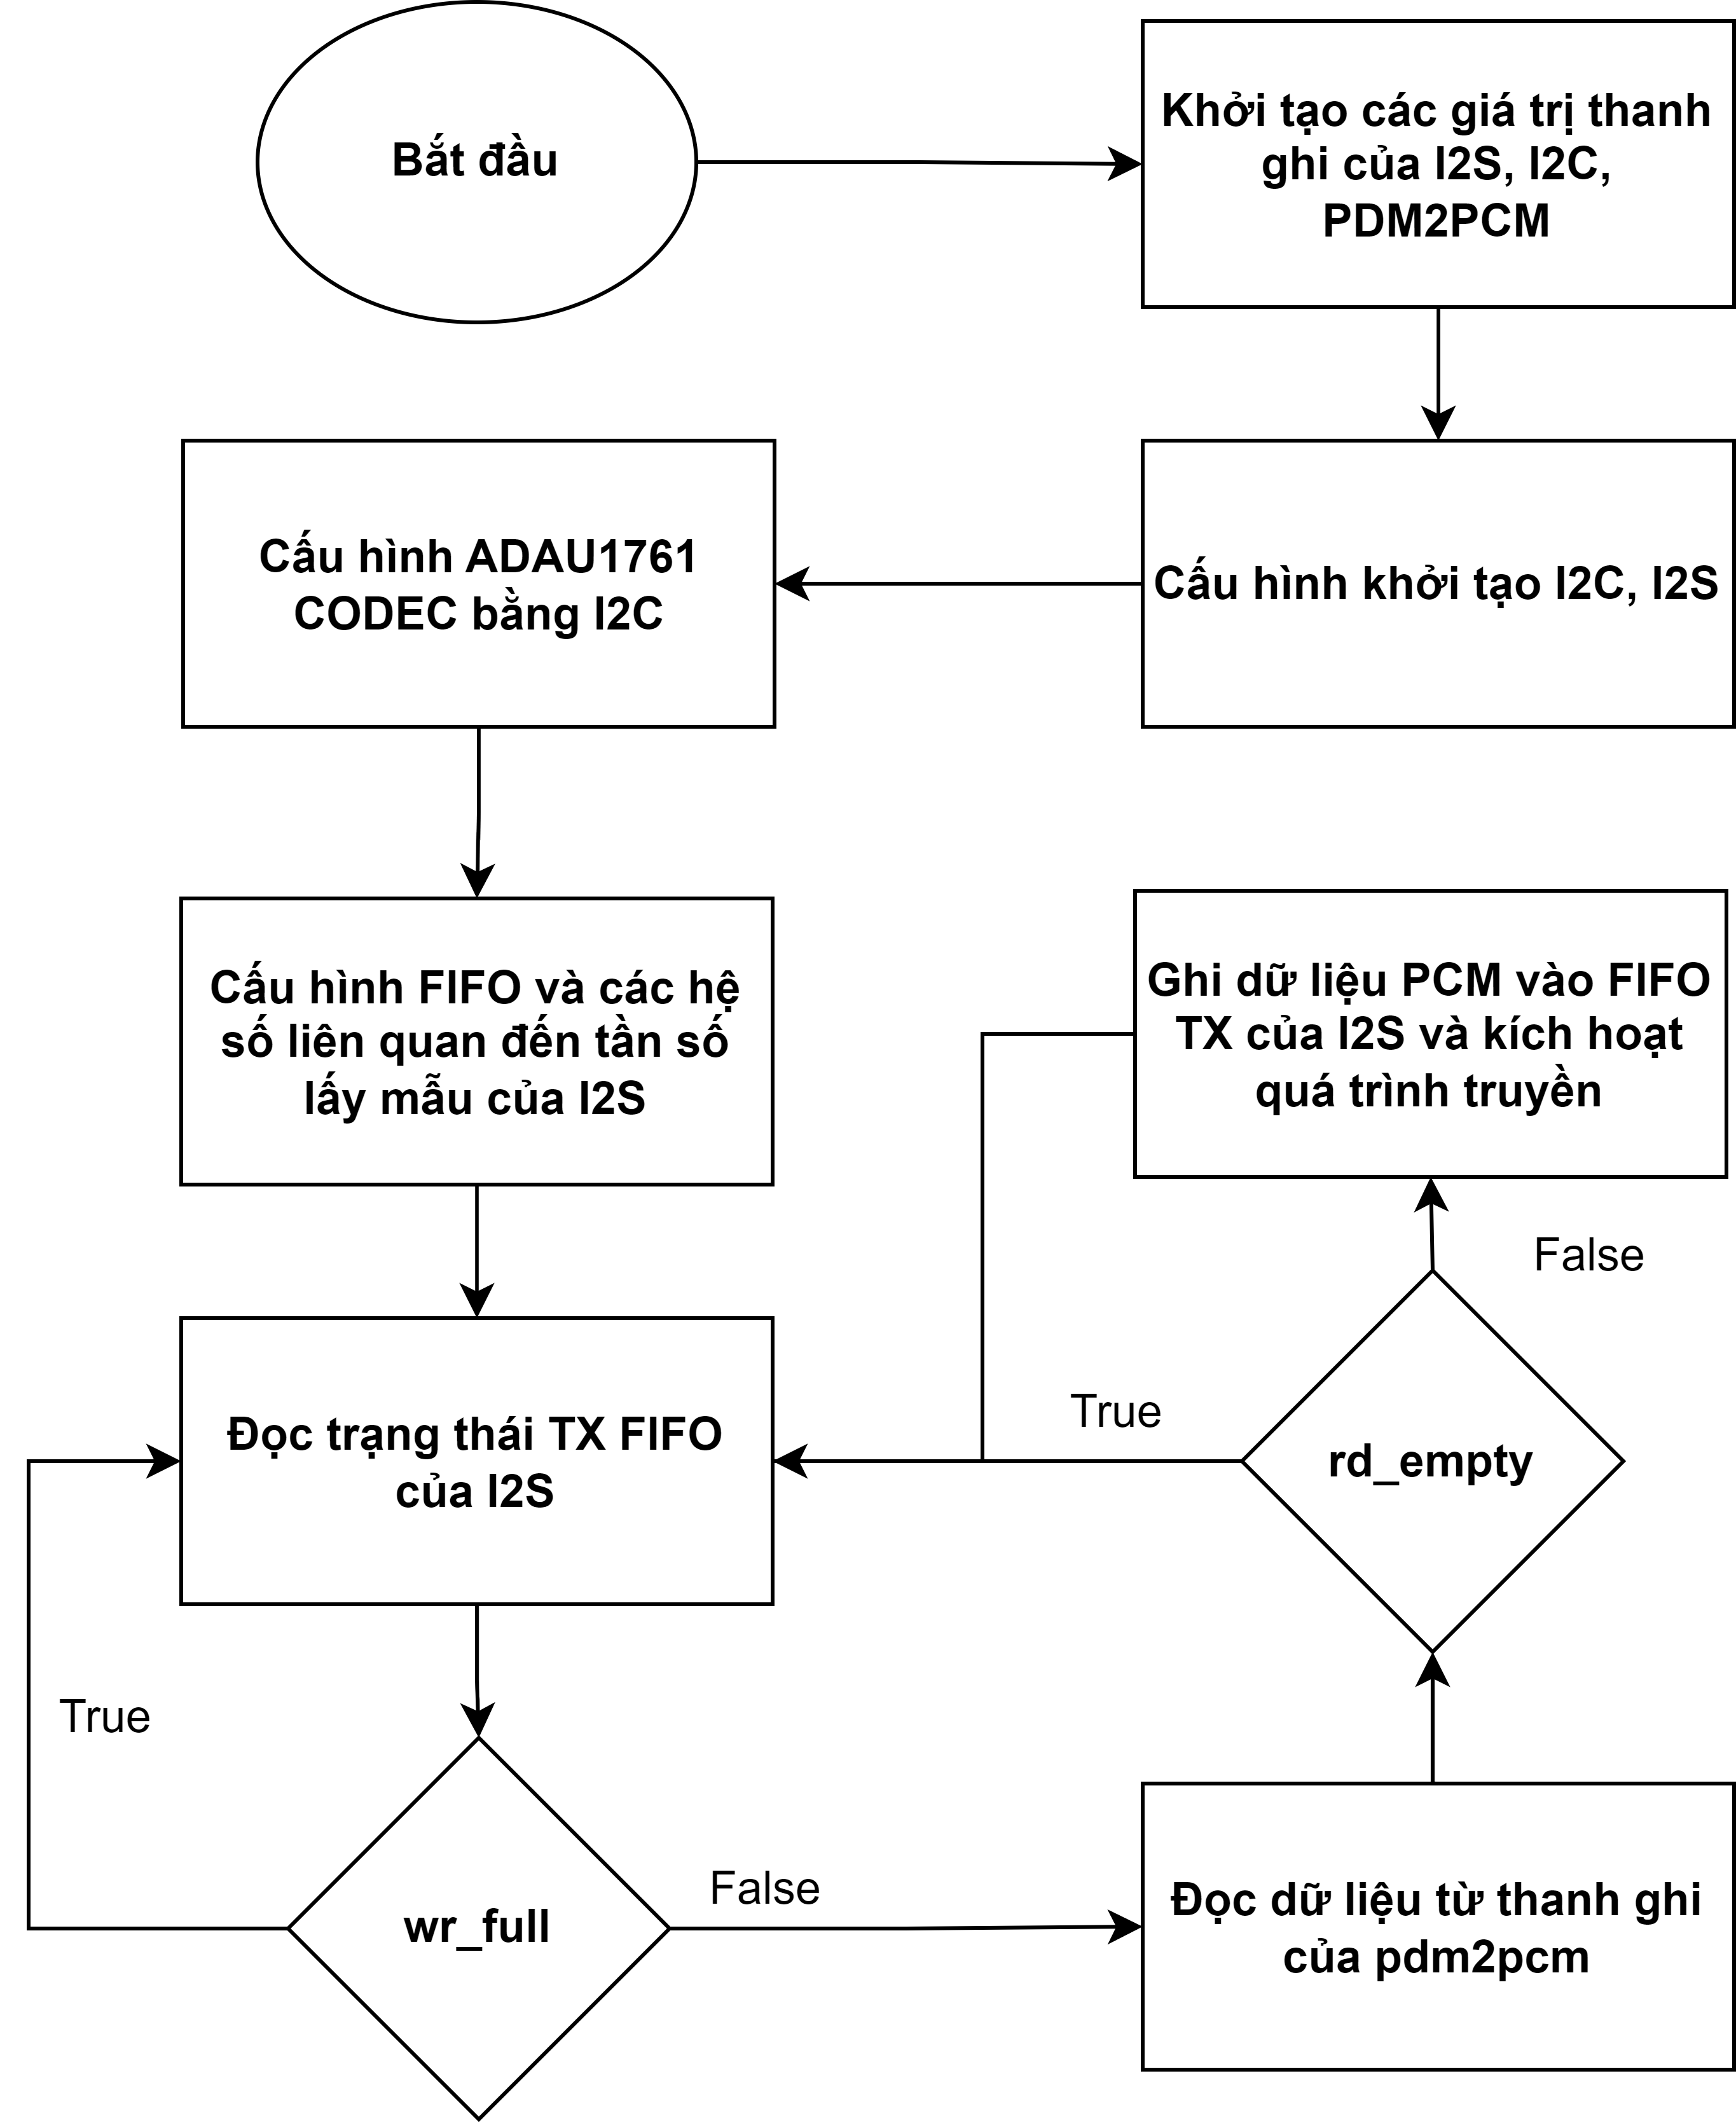
\includegraphics[width=9cm]{Images/Chuong5/fpga/flow_chart.png}
    \caption[Lưu đồ thuật toán của chương trình điều khiển]{\bfseries \fontsize{12pt}{0pt}\selectfont Lưu đồ thuật toán của chương trình điều khiển}
    \label{flow_chart}
\end{figure}

\begin{figure}[H]
    \centering
    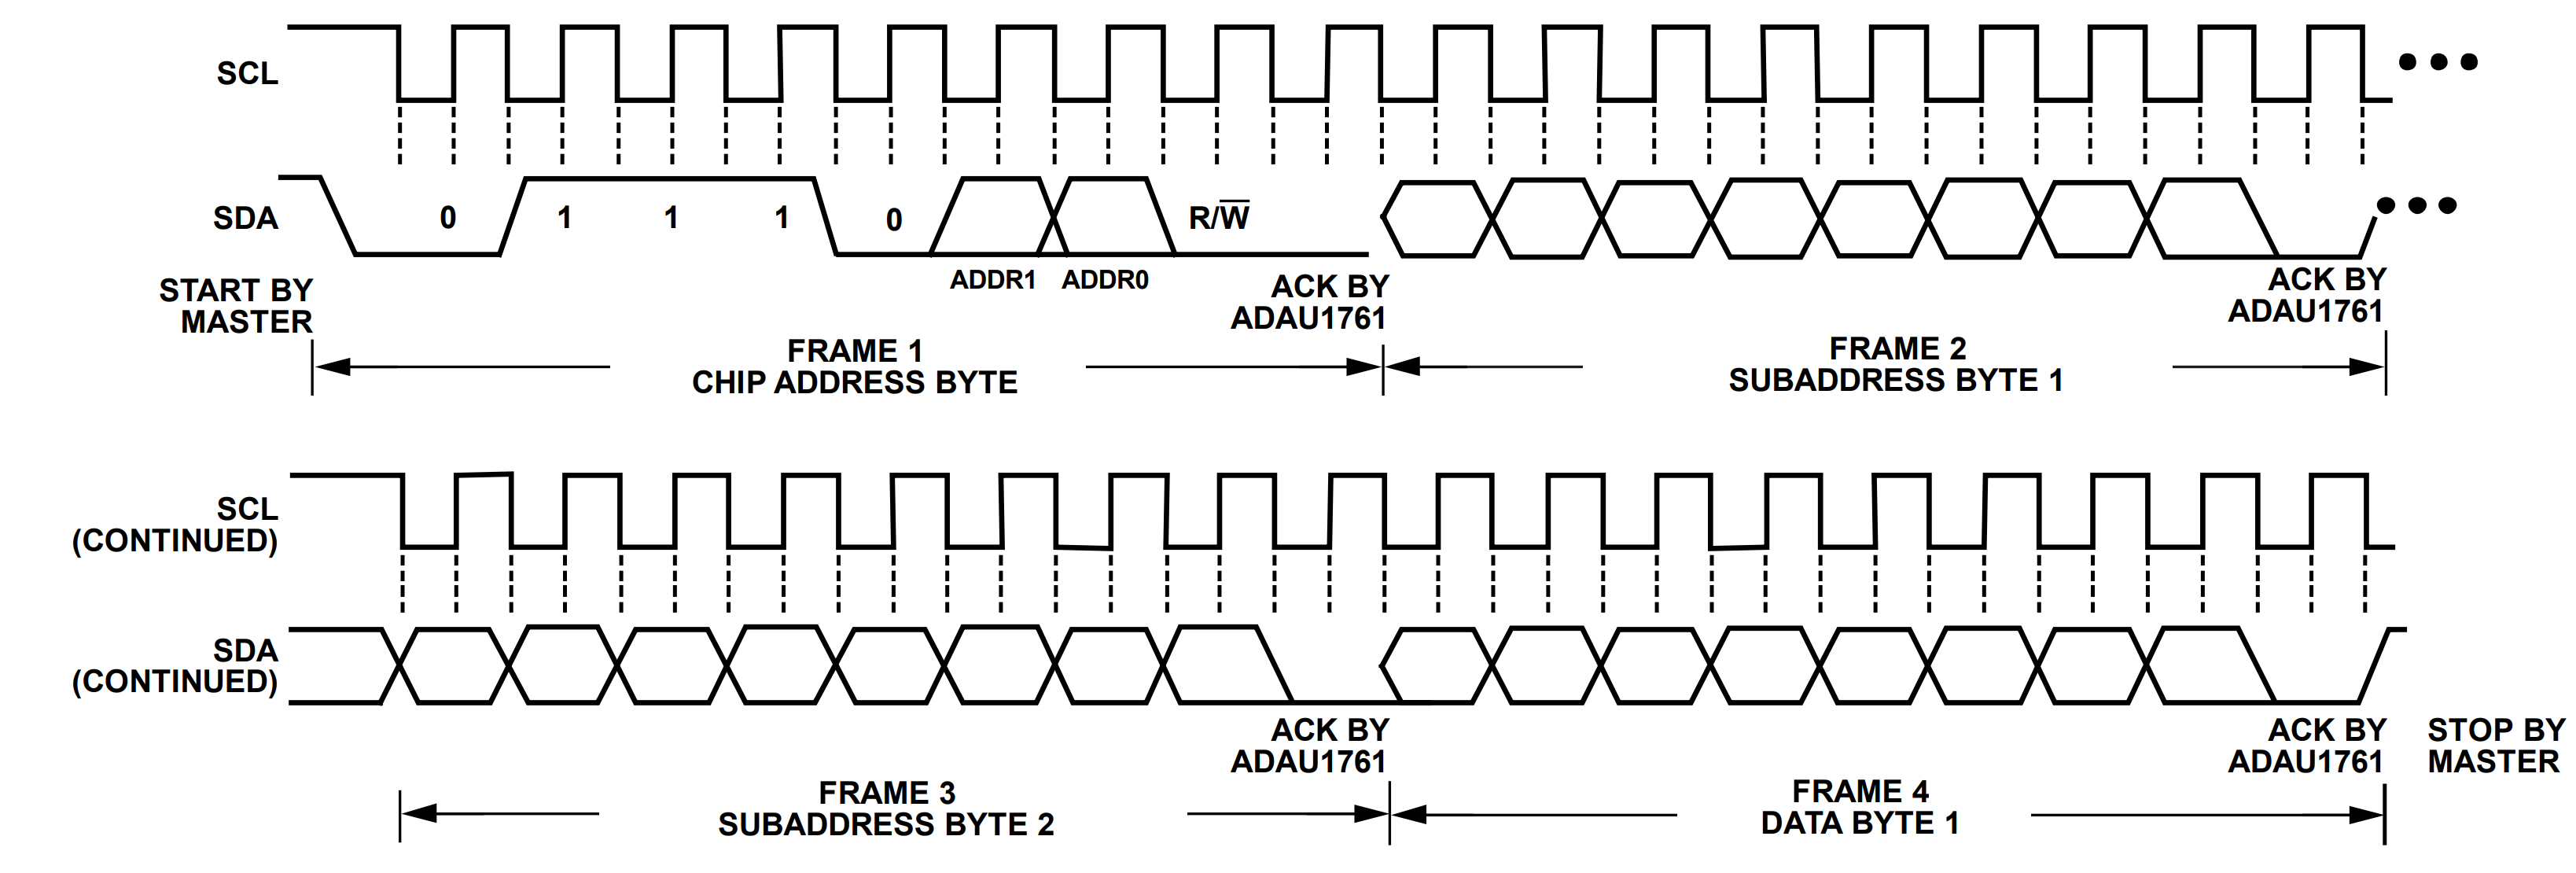
\includegraphics[width=14cm]{Images/Chuong5/fpga/i2c_timing.png}
    \caption[Biểu đồ thời gian theo giao thức I2C để cấu hình chi ADAU1761]{\bfseries \fontsize{12pt}{0pt}\selectfont Biểu đồ thời gian theo giao thức I2C để cấu hình chi ADAU1761}
    \label{i2c_timing}
\end{figure}

Khi đã khởi tạo thành công I2C, chúng ta sẽ tiến hành sử dụng nó để cấu hình cho ADAU1761. Với trình tự một lần chuyển dữ liệu như hình \ref{i2c_timing}, với byte đầu là địa chỉ của slave, 2 byte tiếp theo là địa chỉ phụ (địa chỉ cảu từng thành ghi trong ADAU1761) và byte cuối cùng là dữ liệu. ADAU1761 cung cấp 2 bit ADDR0, ADDR1 để người dùng lựa chọn địa chỉ, với 2 bit này 1 hệ thống có thể có 4 ADAU1716.

Sau khi cấu hình thành công, chúng ta tiến hành quá trình truyền bằng cách kích hoạt các clock của I2S Controler. Việc truyền sẽ lấy dữ liệu từ thanh ghi TX FIFO của I2S.

Hệ thống kiểm tra trạng thái của FIFO trong PDM2PCM thông qua thanh ghi, nếu dữ liệu có tồn tại trong FIFO, vi xử lý tiến hành tách trường dữ liệu PCM trong lần đọc trước đó ghi vào TX FIFO của I2S để truyền với điều kiện trạng thái của TX FIFO không bị đầy. Quá trình này sẽ thực hiện lặp đi lặp lại.

\paragraph{Mô phỏng hệ thống bằng phần mềm QuestaSim}

Testbench lúc này sẽ tích hợp thêm 2 bộ I2C slave và I2S slave để kiểm tra dữ liệu truyền đã thực hiện đúng hay không. 
\begin{figure}[H]
    \centering
    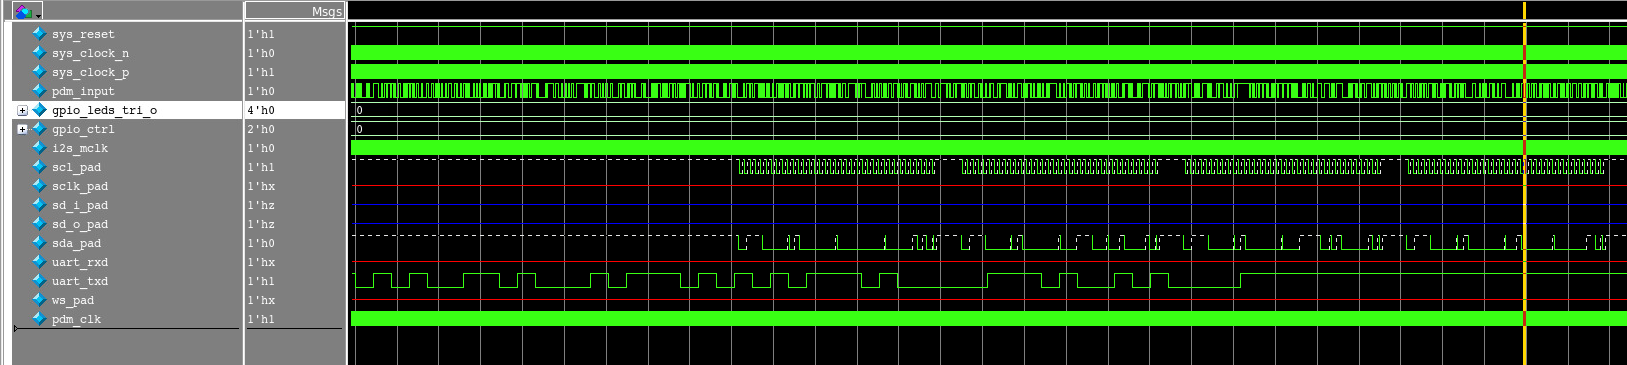
\includegraphics[width=15cm]{Images/Chuong5/fpga/sim_1.png}
    \caption[Kết quả mô phỏng (1)]{\bfseries \fontsize{12pt}{0pt}\selectfont Kết quả mô phỏng (1)}
    \label{sim_1}
\end{figure}
Hình \ref{sim_1} và \ref{sim_2} mô tả kết quả mô phỏng của thiết kế. Tín hiệu đầu ra I2C và I2S thực hiện đúng với các chức năng đã nêu ở mục \ref{code}. dti\_pdm2pcm\_wrapper thực hiện đúng với yêu cầu đặt ra.

\textbf{Kết luận}: việc mô phỏng hoàn toàn chính xác với yêu cầu và chức năng đặt ra.

\begin{figure}[H]
    \centering
    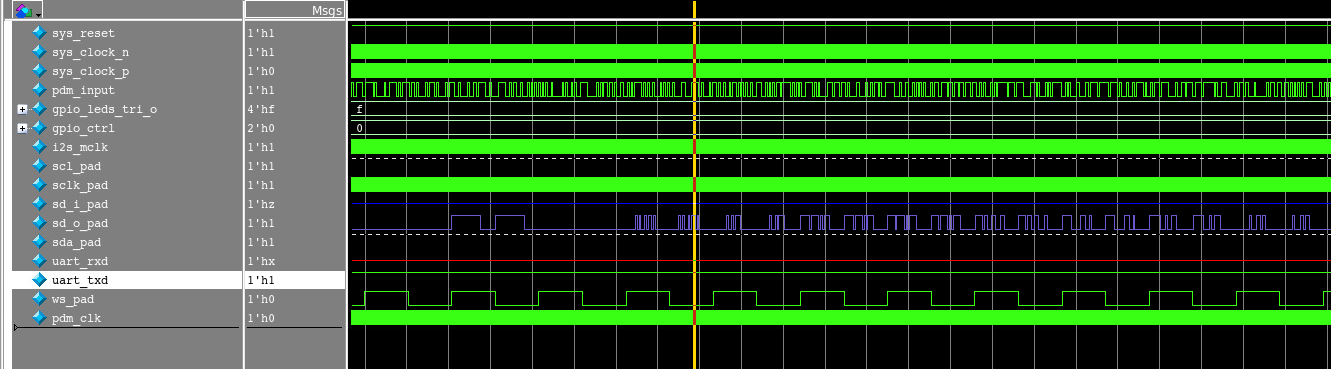
\includegraphics[width=15cm]{Images/Chuong5/fpga/sim_2.png}
    \caption[Kết quả mô phỏng (2)]{\bfseries \fontsize{12pt}{0pt}\selectfont Kết quả mô phỏng (2)}
    \label{sim_2}
\end{figure}


\paragraph{Tổng hợp và triển khai}

Sau khi quá trình mô phỏng đạt kết quả như ý muốn. Chúng ta sẽ bắt đầu quá trình tổng hợp và triển khai.

Các chân của thiết kế sẽ được gán như bảng \ref{constraint}. Kết quả của quá trình tổng hợp mô tả như hình \ref{syn_fpga}, ta có thể thấy LUT chỉ chiếm 14 \% trên số lượng của Zynq-7000.

\begin{table}[H]
\centering
    \caption[Bảng gán chân của thiết kế]{\bfseries \fontsize{12pt}{0pt}\selectfont Bảng gán chân của thiết kế}
   \begin{tabular}{|l|l|l|l|}
\hline
\multicolumn{1}{|c|}{\textbf{Tên}} & \multicolumn{1}{c|}{\textbf{Chiều}} & \multicolumn{1}{c|}{\textbf{Pin}} & \multicolumn{1}{c|}{\textbf{Mô tả}} \\ \hline
sys\_reset               & IN    & F22  & Phím nhấn                    \\ \hline
sda\_pad                 & INOUT & AB5  & chân AC-SDA của ADAU1761     \\ \hline
gpio\_led\_tri\_o{[}3{]} & OUT   & U21  & LED3                         \\ \hline
gpio\_led\_tri\_o{[}2{]} & OUT   & U22  & LED2                         \\ \hline
gpio\_ctrl{[}1{]}        & OUT   & Y5   & chân AC-ADR1 của ADAU1761    \\ \hline
gpio\_ctrl{[}0{]}        & OUT   & AB1  & chân AC-ADR0 của ADAU1761    \\ \hline
i2s\_mclk                & OUT   & AB2  & chân AC-MCLK của ADAU1761    \\ \hline
sys\_clk                 & IN    & Y9   & Tần số 100 MHz               \\ \hline
pdm\_input               & IN    & Y11  & PDM đầu vào                  \\ \hline
gpio\_led\_tri\_o{[}1{]} & OUT   & T21  & LED1                         \\ \hline
gpio\_led\_tri\_o{[}0{]} & OUT   & T22  & LED0                         \\ \hline
sclk\_pad                & INOUT & AA6  & chân BCLK của ADAU1761       \\ \hline
ws\_pad                  & INOUT & Y6   & chân LRCLK của ADAU1761      \\ \hline
sd\_i\_pad               & IN    & AA7  & chân ADC\_SDATA của ADAU1761 \\ \hline
pdm\_clk                 & OUT   & AA11 & Clock của tín hiệu PDM       \\ \hline
sd\_o\_pad               & OUT   & Y8   & chân DAC\_SDATA của ADAU1761 \\ \hline
scl\_pad                 & INOUT & AB4  & chân AC-SCK của ADAU1761     \\ \hline
\end{tabular}
    \label{constraint}
\end{table}


\begin{figure}[H]
    \centering
    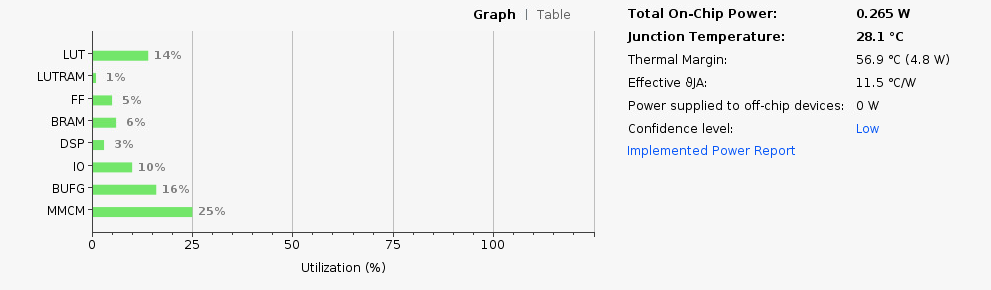
\includegraphics[width=14cm]{Images/Chuong5/fpga/syn_fpga.png}
    \caption[Kết quả tổng hợp trên bằng Vivado]{\bfseries \fontsize{12pt}{0pt}\selectfont Kết quả tổng hợp trên bằng Vivado}
    \label{syn_fpga}
\end{figure}

\subsubsection{Kết quả}

Hình \ref{machthat_2} mô tả mạch triển khai thực tế, sử dụng \textbf{Adafruit PDM Microphone} để thu âm thanh sau đó phát trực tiếp qua loa bằng cổng Line Out 3.5 mm.

\textbf{Nhận xét}: Tín hiệu đã phát được trực tiếp từ micro đến loa. Tín hiệu ổn định không bị rè. Tiến hành kiểm thử hệ thống trong 2 giờ liên tục, thiết bị không bị nóng, hoạt động ổn định. Trong lúc không dùng, tín hiệu phát ra loa không bị rè.

\textbf{Kết luận}: Kết quả truyền nhận trên FPGA thể hiện đúng các chức năng và hoạt động ổn định,.. đảm bảo bộ chuyển đổi làm việc tốt trên các thiết bị thật.


\begin{figure}[H]
    \centering
    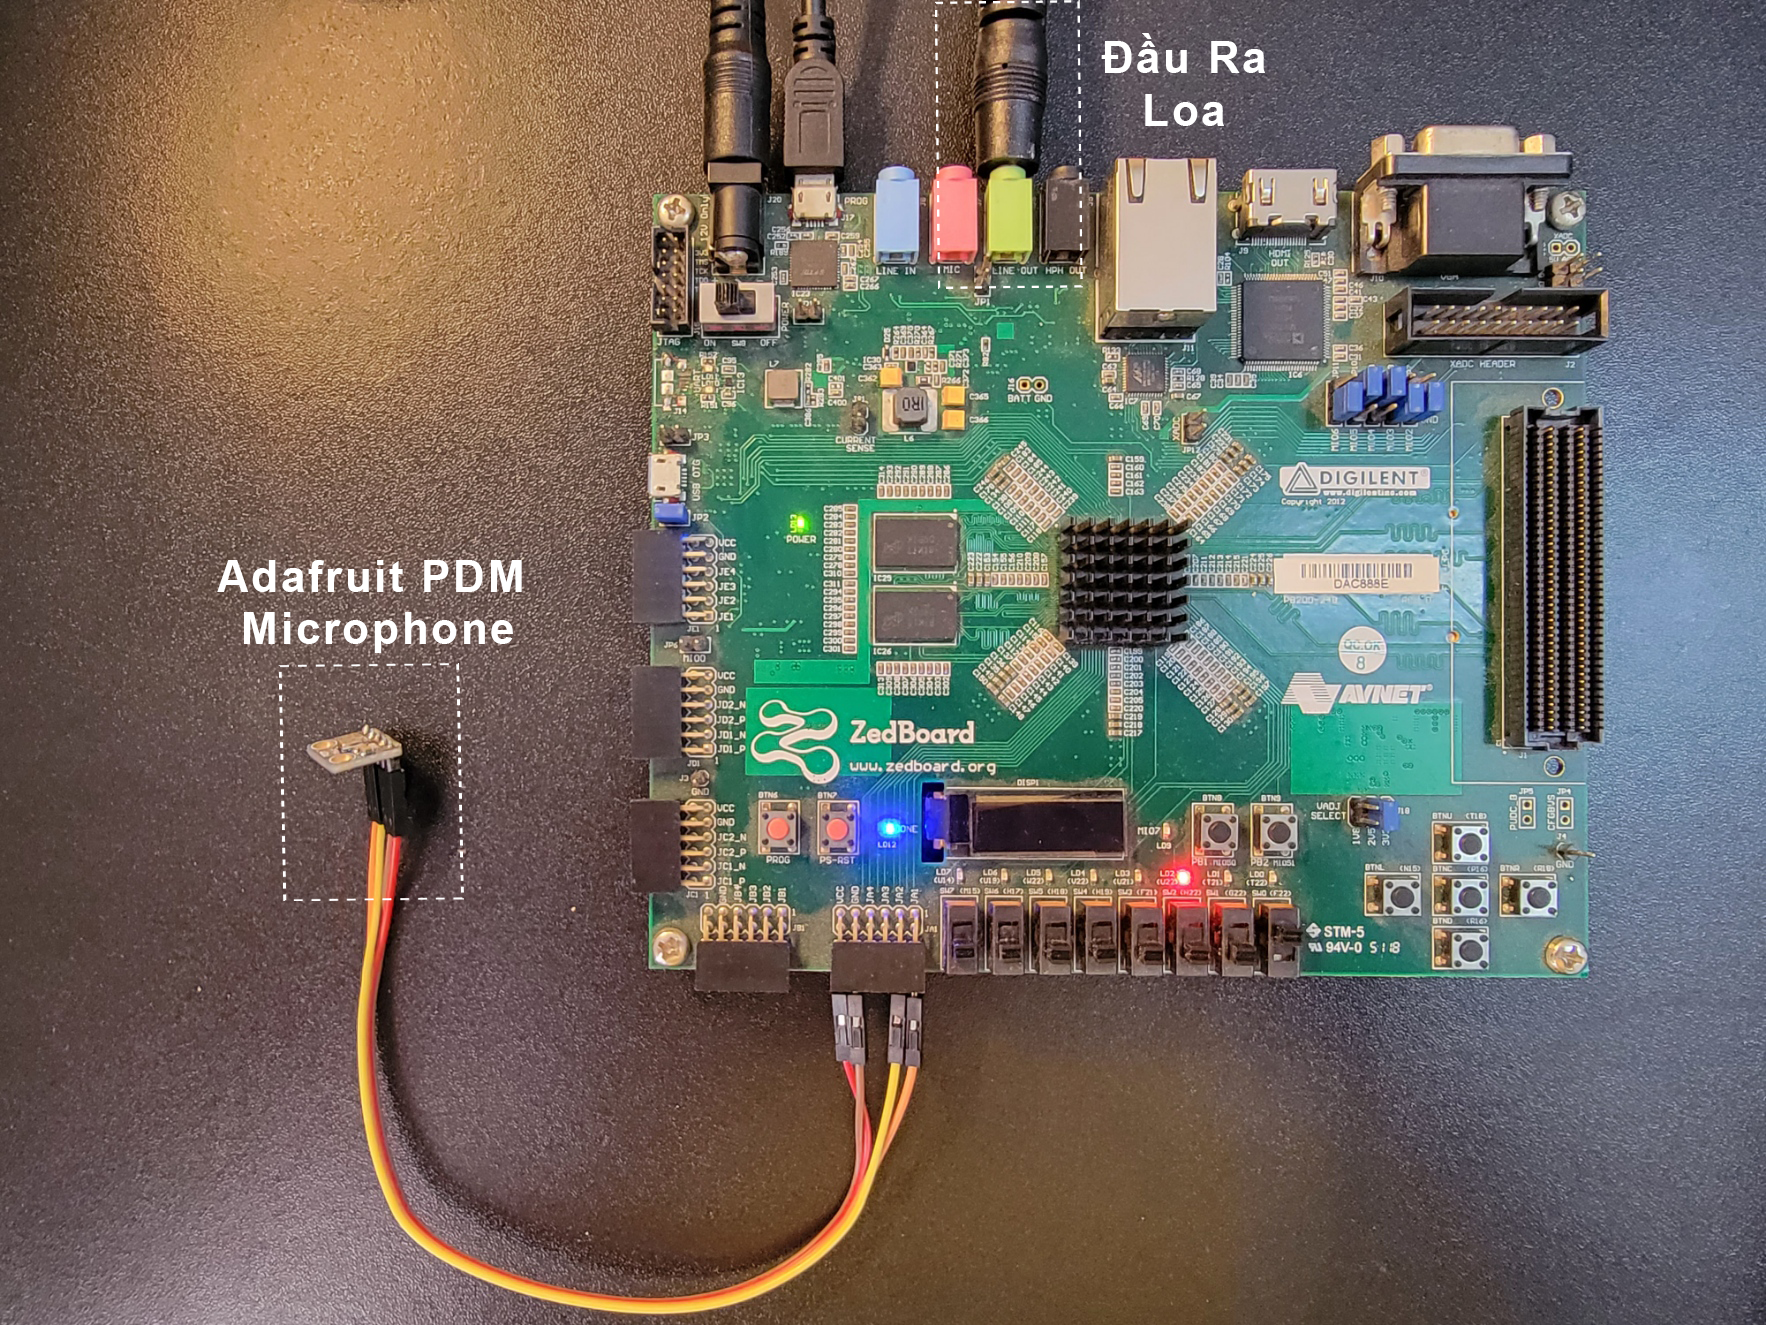
\includegraphics[width=14cm]{Images/Chuong5/fpga/machthat_2.png}
    \caption[Triển khai trên mạch thật]{\bfseries \fontsize{12pt}{0pt}\selectfont Triển khai trên mạch thật}
    \label{machthat_2}
\end{figure}

\subsection{Kết luận chương}

\hyperref[chuong5]{Chương 5} trình bày về quá trình và kết quả của bước tổng hợp và triển khai thiết kế xuống FPGA. Xây dựng kịch bản kiểm thử tương tự như phần mô phỏng, thiết kế block design với các khối tương ứng. Kết quả sau khi triển khai trên FPGA đúng với kết quả dự tính đã đặt ra.
\newpage